\documentclass[times, utf8, zavrsni]{fer}

\usepackage{booktabs}
\usepackage[hidelinks]{hyperref}
\usepackage{float}
\usepackage{pdfpages}
\usepackage{algorithm}
\usepackage{xcolor}
\usepackage{listings}

\definecolor{myblue}{RGB}{68, 114, 196}
\definecolor{mygreen}{RGB}{0, 176, 80}
\lstset{language=Java, tabsize=2}

\begin{document}

% \thesisnumber{6950}
% \title{Klasifikacija uporabom umjetnih neuronskih mreža}
% \author{Darijo Brčina}

% \maketitle

% Ispis stranice s napomenom o umetanju izvornika rada. Uklonite naredbu \izvornik ako želite izbaciti tu stranicu.
%\izvornik
% 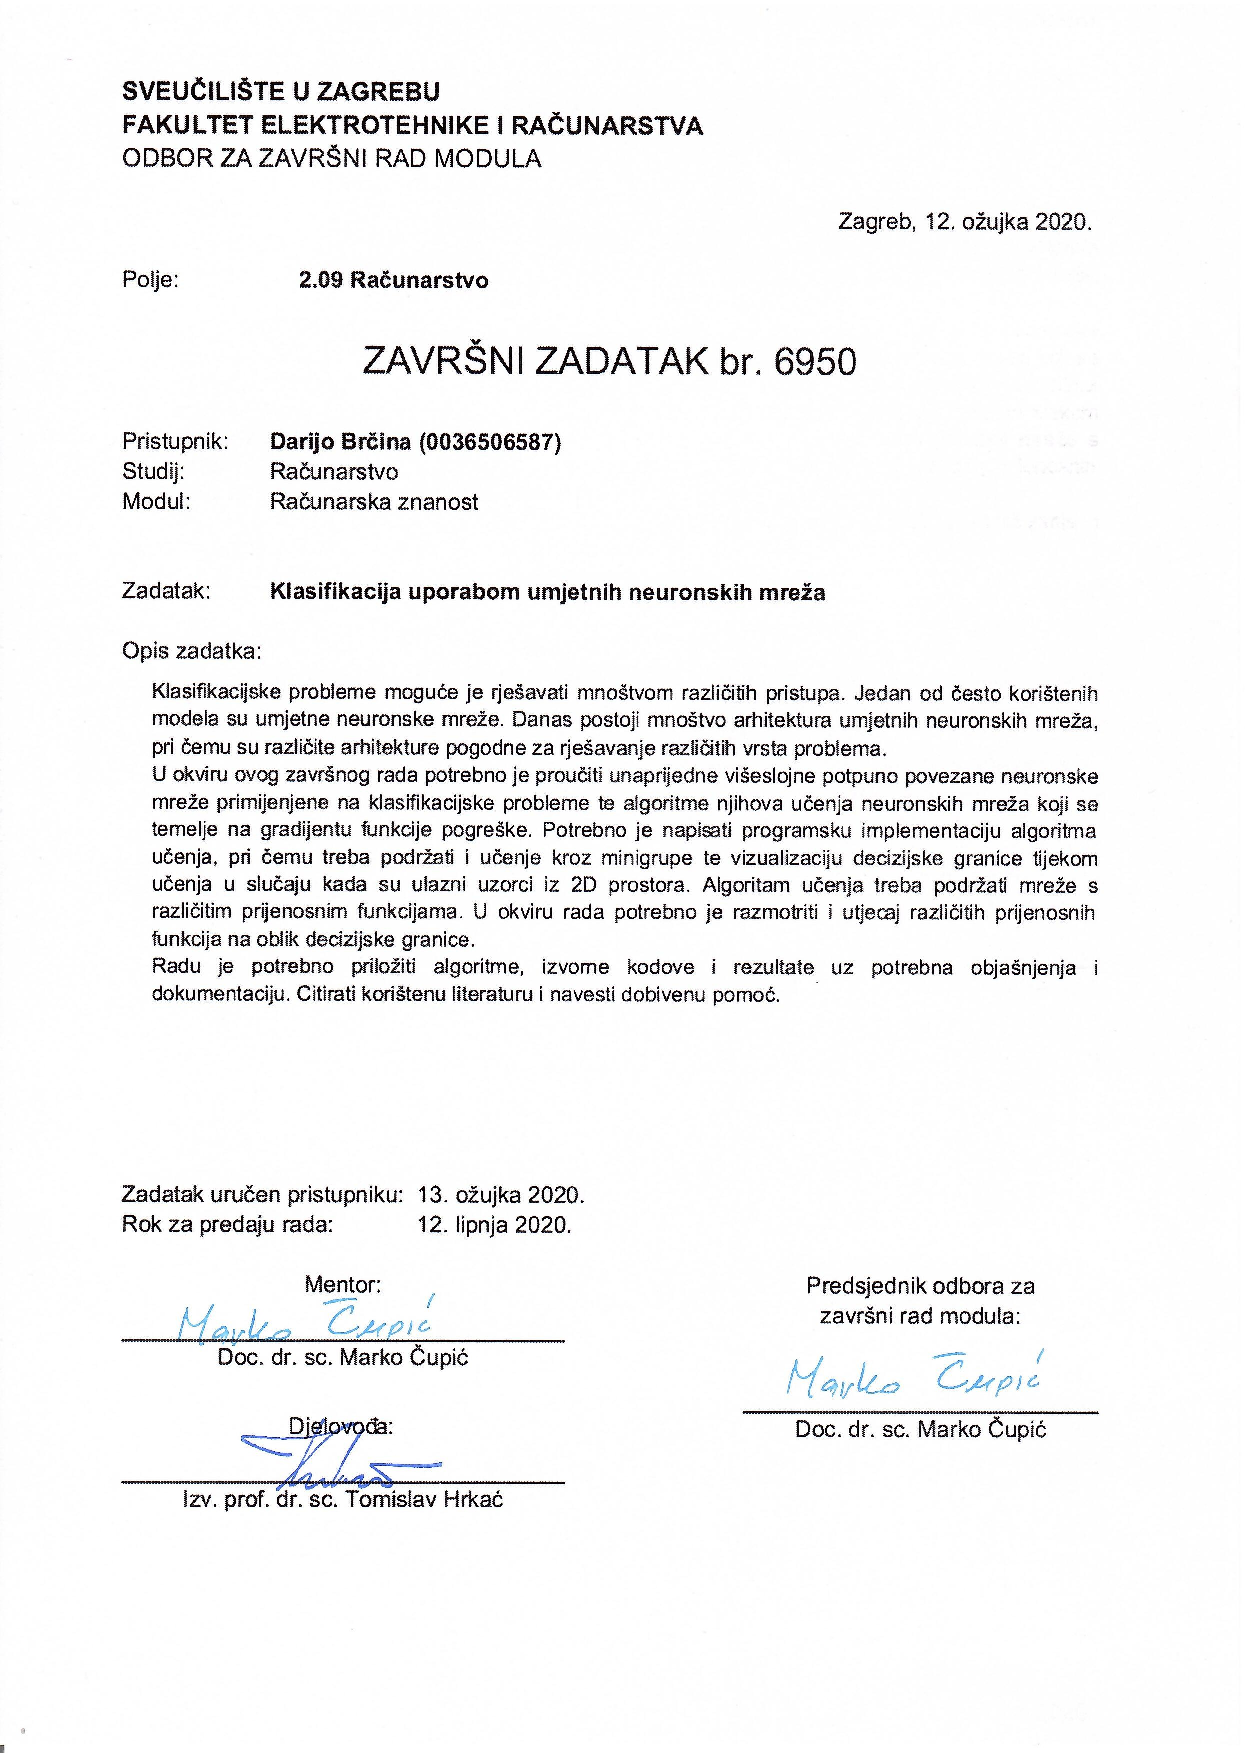
\includepdf[pages=-]{zadatak}

% Dodavanje zahvale ili prazne stranice. Ako ne želite dodati zahvalu, naredbu ostavite radi prazne stranice.
\zahvala{Zahvaljujem mentoru Marku na slobodi odabira teme za ovaj rad i na mnoštvu ukazane literature.}

\tableofcontents

\chapter{Uvod}
Projektiranje sustava koji samostalno uče je osnovni problem moderne računarske znanosti. Sam postupak učenja ne predstavlja toliki problem koliko modeliranje raznih modela koje je potrebno naučiti te odabira dobrog algoritma iz palete mnoštva. Često se moramo pitati što točno želimo da sustav čini te koje onda postupke umjetne inteligencije možemo iskoristiti. Najbanalniji primjer je prepoznavanje sadržaja slike na kojoj se može nalaziti mnoštvo sadržaja. Npr. prepoznavanje rukom pisanih brojeva, razlikovanje ljudi od životinja i neživih stvari itd.

U ovom radu ćemo se dotaknuti teorijske podloge jednog od algoritama umjetne inteligencije, točnije nadziranog učenja, u svrhu kreiranja jednog jednostavnog klasifikatora koji će razviti svojstvo raspoznavanja razreda na temelju 2D koordinata.

\bigskip
U drugom poglavlju dan je kratak pregled područja umjetne inteligencije i strojnog učenja. U trećem poglavlju detaljnije je prikazana teorijska podloga nadziranog učenja. Četvrto poglavlje opisuje algoritam umjetne neuronske mreže kroz povijest do danas te njegova razna svojstva i primjene. U petom poglavlju su prikazani rezultati programske implementacije koji potkrepljuju teoriju četvrtog poglavlja.

\chapter{{Pregled područja}}
Pitate li se ikada što je to inteligencija te čemu nam služi. To pitanje postavljeno je još za vrijeme začetka filozofije kao znanosti kada su se tadašnji filozofi pitali na koji način je ljudsko razmišljanje, učenje i pamćenje ostvareno. Ni dan danas ne postoji jednoznačan odgovor na to pitanje jer ljudski mozak i dalje predstavlja jednu veliku nepoznanicu koja vjerojatno nikada ili ne tako skoro neće biti razriješena. No, znanost je podosta napredovala i shodno tomu se razvila želja da se ljudska inteligencija pokuša pretočiti u nekakvu vrstu inteligencije strojeva.

Početak ovakvog razmišljanja datira od 50-tih godina dvadesetog stoljeća kada Alan Turing u članku \textit{Computing Machinery and Intelligence} časopisa \textit{Mind} postavlja pitanje: Mogu li strojevi misliti? \engl{Can machines think?} na koje pokušava odgovoriti kroz tzv. igru imitacije \engl{imitation game}. Sudionici igre su tri igrača: igrač A, igrač B i igrač C gdje su igrači A i B ispitanici, a igrač C ispitivač. Cilj igrača C je utvrditi spol ispitanika postavljanjem pitanja, cilj igrača B je pomoći ispitivaču C, a cilj igrača A je navesti ispitivača C na pogrešnu identifikaciju. Što će se dogoditi ako stroj uzme mjesto igrača A? Ako broj pogrešaka igrača C bude gotovo jednak u oba slučaja, onda je stroj inteligentan \citep{turingAI}. Ovakav princip testiranja se često naziva Touringov test \engl{Turing test}.

Nedugo nakon Touringov eksperimenta 1956.\ se održava konferencija u Dartmouthu \citep{wiki:DART} na inicijativu John McCarthy-a, tadašnjeg mladog profesora matematike na fakultetu u Dartmouthu, koji okuplja oko sebe nekolicinu znanstvenika i prijatelja kako bi pokušali koncepte ljudske inteligencije preslikati u inteligenciju strojeva. Cilj je pokazati kako strojevi koriste jezik, kako zaključuju i stvaraju apstraktne koncepte i kako vremenom postaju sve prilagodljiviji na predočene probleme baš kao i ljudi. Inicijalna ideja je bila da se neki od navedenih problema može dokazati uz manju skupinu dobrih znanstvenika i kroz period od jednog ljeta (McCarthy et al. 1955). To naravno nije bilo moguće. Time se formalno uvodi pojam \textit{umjetna inteligencija}.

\section{Umjetna inteligencija}
Kao što je anticipirano ranije, umjetna inteligencija \engl{artificial intelligence} je laički rečeno inteligencija strojeva, a znanost koja se bavi proučavanjem umjetne inteligencije naziva se računarska znanost \engl{computer science}.

Primjena umjetne inteligencije danas je izrazito rasprostranjena kroz gotovo svaku industriju. Pronalazimo ju u medicini, automobilskoj industriji, robotici, pa i u sportskoj i industriji igara. Jedan od poznatijih događaja koji prikazuje primjenu umjetne inteligencije dogodio se 2016.\ kada je računalo naziva \textit{AlphaGo} u igri \textit{Go} uspjelo pobijediti svjetskog prvaka Lee Sedolu rezultatom 4:1 te time ostvario veliki uspjeh u svijetu umjetne inteligencije kao i pažnju javnosti \citep{moyerGO}.

Umjetnu inteligenciju je dakako potrebno trenirati i učiti pa je tako učenje podijeljeno na dvije veće cjeline:
\begin{center}
    \begin{enumerate}
        \item simboličko učenje i
        \item strojno učenje.
    \end{enumerate}
\end{center}

\subsection{Simboličko učenje}
Simbolička umjetna inteligencija \engl{symbolic artificial intelligence} je izraz koji definira skup istraživačkih metoda koje se temelje na ljudima lako čitljivim simbolima \engl{human-readable simbols} koji modeliraju probleme i logiku. Jedan od najboljih primjera jesu \textit{ekspertni sustavi} \engl{expert systems} koji se temelje na skupu pravila. Pravila su modelirana na sličan način kao i "ako-onda" rečenica \engl{if-then statement} koja je u ljudskoj komunikaciji svakodnevno u upotrebi. Također, razne vrste logika poput propozicijska \engl{Propositional logic}, često referirana kao Booleova algebra, logika prvog reda \engl{First order logic}, poznatija kao predikatna logika \engl{Predicate logic} i neizrazita logika \engl{Fuzzy logic} pripadaju upravo simboličkoj umjetnoj inteligenciji. Ovakav način učenja bio je popularan početkom 1950.\ sve do kraja 1980.\ \citep{wiki:SIMB}.

\subsection{Strojno učenje}
Strojno učenje \engl{Machine learning, ML} predstavlja niz metoda i algoritama koji sustavima pružaju stjecanje novog znanja kroz modeliranje obrazaca koje onda kasnije mogu iskoristiti za predviđanje novih podataka ili sličnih \citep{cupicML}. Glavna ideja je da sustavi uče iz iskustva, empirijski, bez da se programska implementacija mijenja, što znatno olakšava manipulaciju istih.

Danas postoji nezgrapno puno podataka koje je moguće i koje je potrebno iskoristiti za učenje pa je cilj konstruirati sustave koji mogu iskoristiti baš te podatke za neka korisna ponašanja poput predviđanja i raspoznavanja raznih uzoraka \citep{cupicML}. Podatci se svrstavaju u dvije grupe: \textit{numerički} i \textit{kategorički} podatci. Numerički podatci su svi oni podatci nad kojima je moguće izvršiti aritmetičke operacije. Npr. unos dnevnih kalorija, broj slobodnih bacanja na košarkaškoj utakmici, isplata plaća i sl. Kategorički podatci se dodatno dijele u dvije podgrupe: \textit{nominalni} i \textit{ordinalni} podatci. Nominalni podatci su imenovani podatci koji nisu numerički, tj.\ podatci nad kojima nisu definirane aritmetičke operacije. Npr.\ podatci o spolu jedinke, osjećaju raspoloženja poput "tužan" ili "veseo" i sl.\ Ordinalni podatci također nemaju definiranu aritmetiku, no imaju definiran prirodan poredak i mogu se uspoređivati. Npr.\ mišljenje jedne osobe može biti "jako zadovoljan", dok druge "zadovoljan", što možemo usporediti i konstruirati prirodan poredak.

Strojno učenje dijelimo na četiri područja:
\begin{center}
    \begin{enumerate}
        \item nadzirano učenje,
        \item nenadzirano učenje,
        \item polu-nadzirano učenje i
        \item podržano učenje.
    \end{enumerate}
\end{center}

\textit{Nadzirano učenje} je tema ovog rada pa će biti obrađeno detaljnije u narednom poglavlju.

\bigskip

\textit{Nenadzirano učenje} \engl{Unsupervised learning} je vrsta učenja u kojem skup uzoraka predstavljaju samo ulazni podatci bez znanja o tome kako bi isti trebali biti tabelirani. Zbog ovakvog pristupa, učenje je dobilo ime nenadzirano učenje, tj.\ učenje bez prisustva učitelja \engl{supervisor}. Najpoznatiji postupak nenadzirano učenja je postupak grupiranja \engl{clustering}. Cilj grupiranja je na temelju danih uzoraka pokušati pronaći sve uzorke koji imaju slična svojstva te ih zatim grupirati u odvojene razrede. Npr.\ neka skup ulaznih uzoraka sustava bude mješavina slika ljudi i slika automobila. Kao konačni rezultat, moraju se stvoriti dva razreda: razred ljudi te razred automobila. Na slici \ref{fig:clustering} prikazan je primjer grupiranja.

\begin{figure}[H]
    \centering
    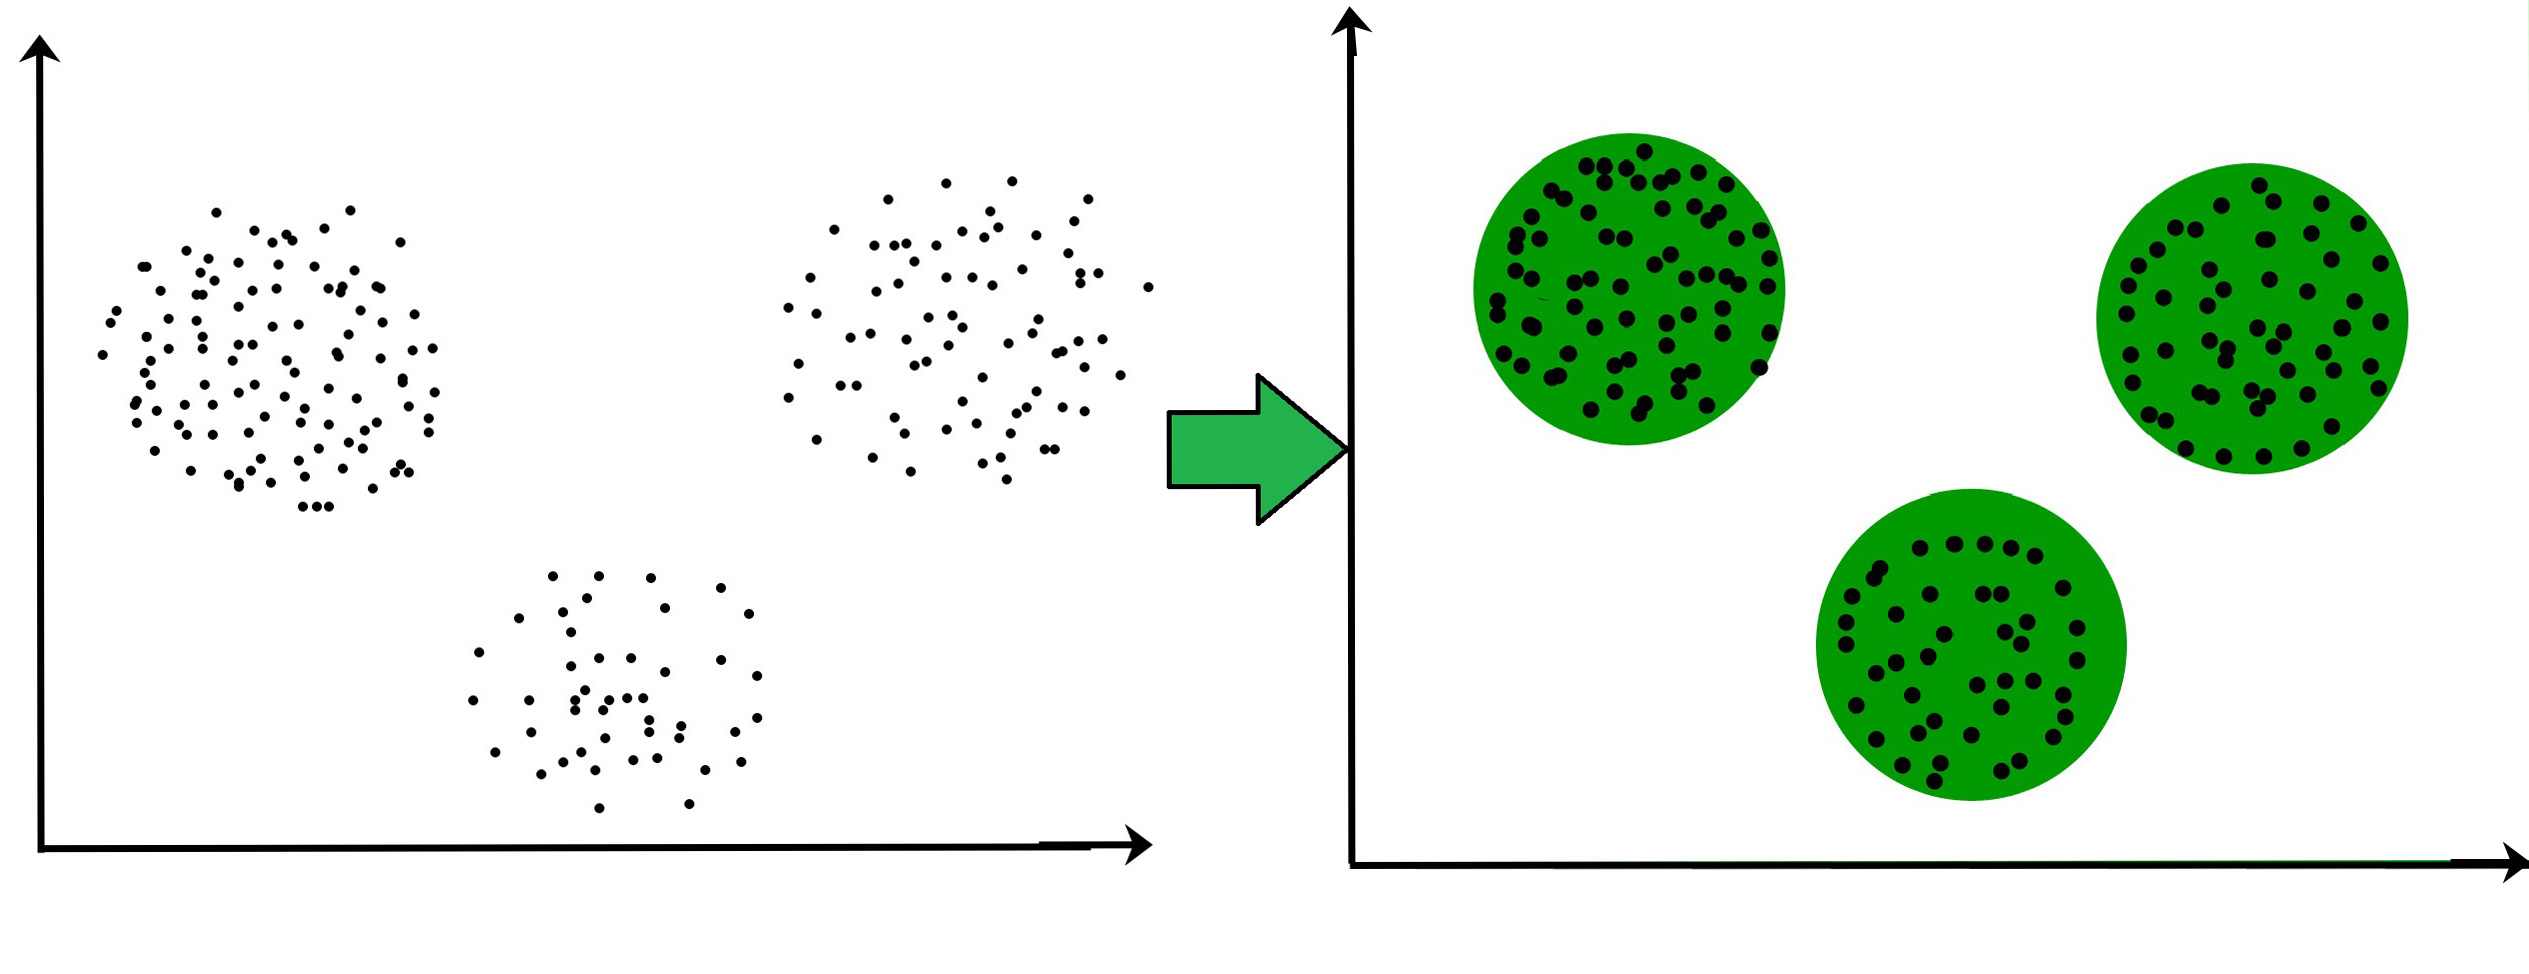
\includegraphics[scale=0.75]{img/clustering.jpg}
    \caption[Caption for LOF]{Primjer grupiranja\footnotemark}
    \label{fig:clustering}
\end{figure}
\footnotetext{Preuzeto sa https://www.geeksforgeeks.org/clustering-in-machine-learning/ [Pristupljeno 10-Maj-2020].}

Uz grupiranje poznati postupci su i postupci smanjenja dimenzionalnosti \engl{dimensionality reduction}, postupci otkrivanja stršećih ili novih vrijednosti \engl{outlier detection, novelty detection} i drugi.

\bigskip

\textit{Polu-nadzirano učenje} \engl{Semi-supervised learning}, kao što samo ime nalaže, je učenje u kojem se isprepliću koncepti nadziranog učenje s konceptima nenadziranog učenja. Ono pokazuje dosta veće uspjehe nego navedeni, no izvedba je izrazito zahtjevnija \citep{wiki:SEMISUP}.

\bigskip

\textit{Podržano učenje} \engl{Reinforcement learning, RL} je vrsta učenja koja se potpuno razlikuje od svih do sada navedenih jer ono ne očekuje nikakve tabelirane ulazne ili izlazne podatke već je glavna ideja optimizacija ponašanja računalnih agenata. Razmatra se interakcija agenta s okolinom \engl{environment} kroz niz akcija za koje isti može biti nagrađen ili kažnjen, ovisno o ishodu akcije. Željeni cilj agenta je maksimizirati mogući dobitak nagrade \citep{wiki:RL}. Na slici \ref{fig:reinforcement-learning} prikazan je model podržanog učenja.

\begin{figure}[H]
    \centering
    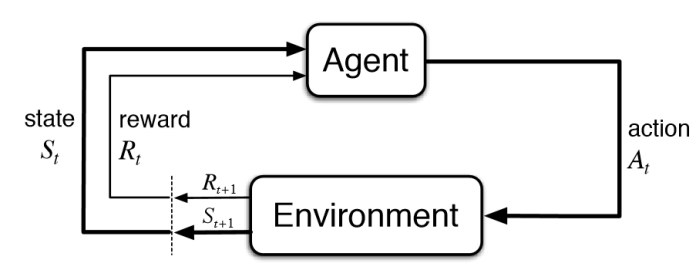
\includegraphics[scale=0.7]{img/reinforcement-learning.jpg}
    \caption[Caption for LOF]{Model podržanog učenja\footnotemark}
    \label{fig:reinforcement-learning}
\end{figure}
\footnotetext{Preuzeto sa https://www.kdnuggets.com/2018/03/5-things-reinforcement-learning.html/ [Pristupljeno 10-Maj-2020].}

\chapter{Nadzirano učenje}
Nadzirano učenje \engl{Supervised learning} je vrsta učenja čiji je cilj sve uzorke koji dođu na ulaz sustava preslikati u izlaz koji točno odgovara predanim ulazima. Dakle, prije samog učenja poznati su ulazi, koji su često modelirani vektorima, te izlazi koji su pridruženi tim ulazima, stoga se tijekom učenja u svakom trenutku zna željeni izlaz te se za krive rezultate daje određena povratna informacija \engl{feedback} o tome koliko sustav griješi. Upravo zbog navedenog koncepta je učenje i dobilo ime nadzirano učenje jer se proces učenja izvršava uz prisustvo učitelja. Razlikujemo dvije faze strojnog modela prikazane na slici \ref{fig:supervised-learning-flow}:
\begin{enumerate}
    \item faza učenja modela i
    \item faza iskorištavanja modela.
\end{enumerate}

\section{Učenje modela}

\begin{figure}[H]
    \centering
    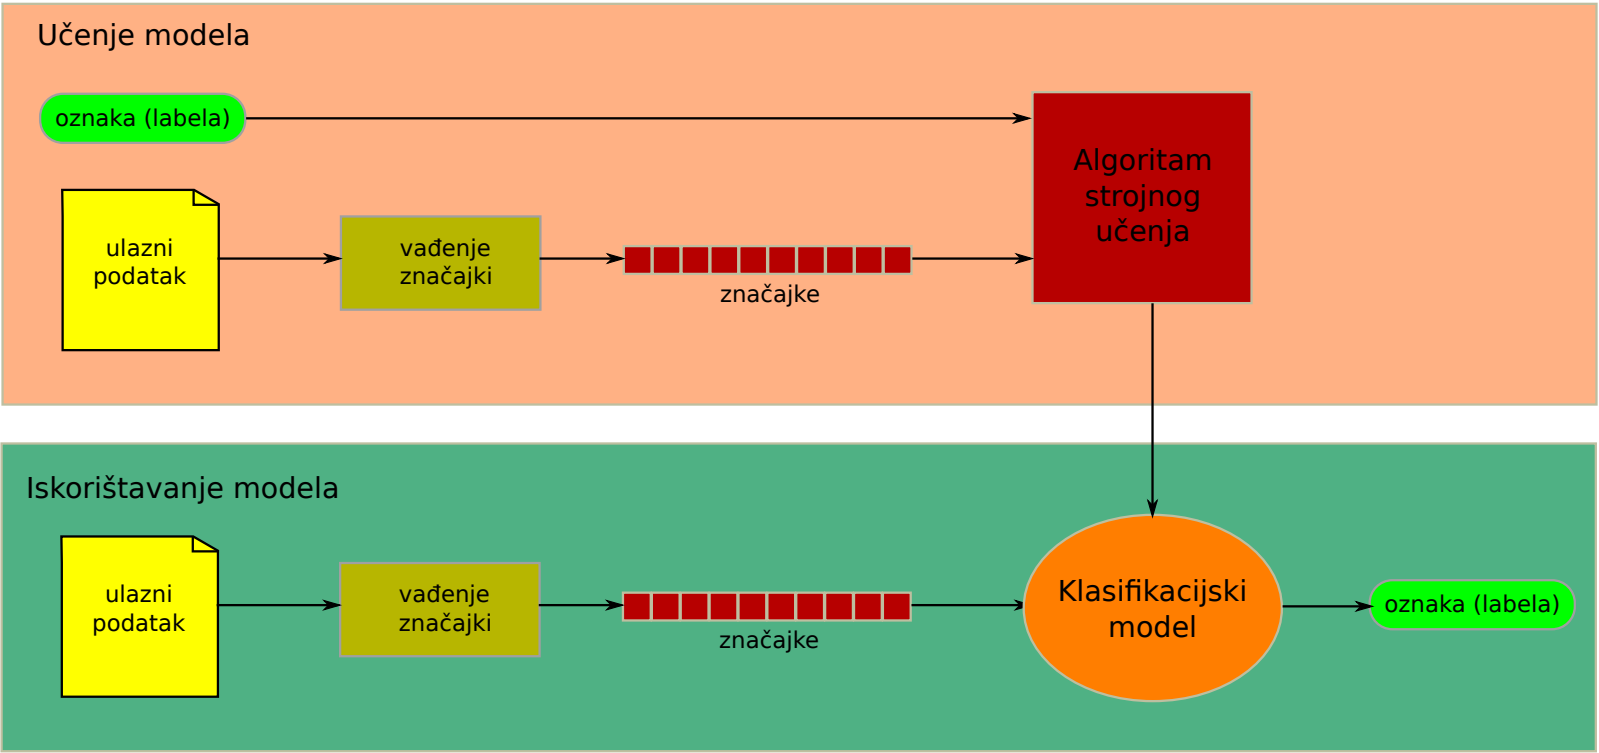
\includegraphics[scale=0.5]{img/supervised-learning-flow.png}
    \caption[Caption for LOF]{Model strojnog učenja\footnotemark}
    \label{fig:supervised-learning-flow}
\end{figure}
\footnotetext{Preuzeto iz literature \citep{cupicML}.}

Tijekom faze učenja, modelu se predaje skup uzoraka za učenje \engl{training set}. Svaki uzorak skupa možemo notirati kao $(\textbf{x}, y)\textsubscript{i}$ što predstavlja \textit{i}-ti uzorak iz skupa za učenje gdje \textbf{x} predstavlja vektor ulaznih podataka, a \textit{y} vrijednost pridružena ulaznom vektoru, odnosno oznaku \engl{label}. Ulazni podatak često može biti kompleksne naravi što znači da ga je potrebno "razbiti" u manje cjeline. Takav postupak se naziva vađenje značajki \engl{feature extraction}. Rezultat navedenog je kolekcija značajki koja se zatim predaje određenom algoritmu strojnog učenja. Npr.\ ulazni podatci mogu biti razne gume poput gume automobila, gume bicikla, gume traktora i sl.\ , a značajka bi onda mogla biti volumen gume, oblik gume, boja gume i sl. Algoritam strojnog učenja će na temelju predanih značajki pokušati optimizirati parametre odabranog modela kako bi se isti mogao koristiti u sljedećoj fazi.

Faza iskorištavanja modela predstavlja fazu u kojoj se treba utvrditi radi li naučeni model s uzorcima nad kojima nije učio, tj.\ je li razvio sposobnost generalizacije \engl{generalization}. Ako model dodijeli točnu oznaku za većinu ulaznih podataka, onda možemo reći da je razvio svojstvo generalizacije. No što ako u velikoj mjeri ne uspije točno povezati izlaze s ulazima? Ako dođe to takve pojave, kažemo da je model pretreniran \engl{overfitting}. Do navedene pojave dolazi kada model nauči previše nad skupom uzoraka za učenje, tj.\ uzorke za učenje nauči savršeno raspoznavati dok za nove uzorke ne uspijeva dati željene rezultate. Postoji nekoliko načina kako se može utjecati da model razvije svojstvo generalizacije, a spomenut ćemo samo jedan od njih, \textit{unakrsna provjera}.

Unakrsna provjera \engl{cross-validation} je postupak koji se koristi tijekom faze učenja modela. Ideja je da se dio uzoraka iz skupa za učenje razdijeli u novi skup, skup za provjeru \engl{validation set}. Skup za provjeru često sadrži od 20\% do 30\% svih uzoraka iz skupa za učenje \citep{cupicML}. Tijekom faze učenja modela, model će i dalje učiti samo nad skupom za učenje, dok ćemo mu povremeno dati i podatke iz skupa za provjeru čisto da se vidi koliko griješi nad njima. Važno je napomenuti da model nad uzorcima iz skupa za provjeru neće učiti, tj.\ neće optimizirati parametre, već će biti prisiljen da nauči generalizirati. Postavlja se pitanje do kada će faza učenja modela onda trajati i odgovor je vrlo jasan. Trajat će do trenutka kada pogreška nad skupom za provjeru počinje rasti. Dijagram na slici \ref{fig:cross-validation} prikazuje kako model uči kroz epohe\footnote{Epoha je ništa drugo nego jedna iteracija učenja, ali u strojnom učenju se često koristi izraz epoha pa ćemo se držati konvencije.}.

\begin{figure}[H]
    \centering
    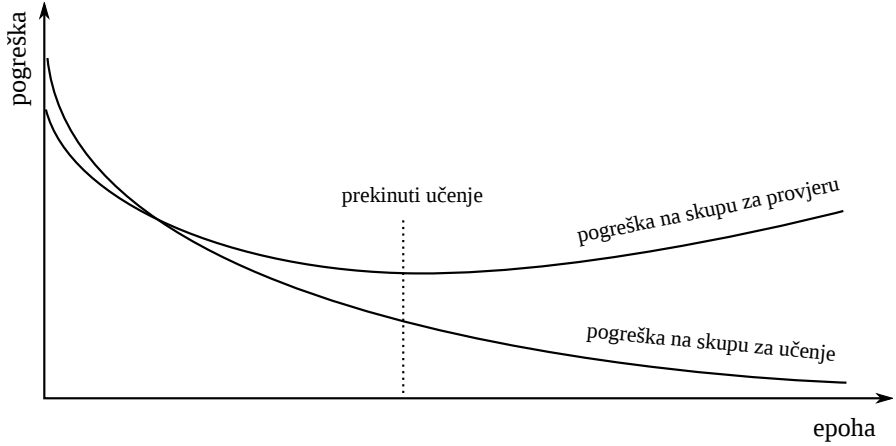
\includegraphics[scale=0.5]{img/cross-validation.png}
    \caption[Caption for LOF]{Kretanje pogrešaka pri učenju strojnog modela\footnotemark}
    \label{fig:cross-validation}
\end{figure}
\footnotetext{Preuzeto iz literature \citep{cupicANN}.}

Također, postoji mogućnost da neki od parametara modela utječu na njegovu složenost. Shodno tomu se uvodi još jedan skup, skup za testiranje \engl{testing set}. Ideja je sljedeća: skup podataka razdijelimo u sva tri do sada navedena skupa i normalno provedemo fazu učenja modela uz malu promjenu. Umjesto da se zadovoljimo samo jednim naučenim modelom, pokušavamo pronaći onaj model koji će najbolje minimizirati pogrešku nad skupom za testiranje \citep{cupicML}.

\section{Problemi nadziranog učenja}
Zadatak nadziranog učenja je sljedeći: pretpostavimo da imamo skup za učenje koji se sastoji od \textit{N} različitih parova ulaza i izlaza;
\[(\textbf{x}\textsubscript{1}, y\textsubscript{1}), (\textbf{x}\textsubscript{2}, y\textsubscript{2}),
(\textbf{x}\textsubscript{3}, y\textsubscript{3}),\dots,
(\textbf{x}\textsubscript{N}, y\textsubscript{N})\]
gdje \textbf{x\textsubscript{i}} predstavlja \textit{i}-ti vektor ulaznih podataka, dok \textit{y\textsubscript{i}} \textit{i}-ti željeni izlaz koji je generiran nekom nepoznatom funkcijom $y=f(\textbf{x})$. \newline
Potrebno je pronaći takvu funkciju \textit{h} koja će najbolje aproksimirati funkciju \textit{f}.

Funkcija \textit{h} naziva se hipoteza \engl{hypothesis} i pripada nekom skupu svih hipoteza \textbf{H} koje donekle aproksimiraju zadanu funkciju \textit{f}, neke bolje, neke lošije. U ovom trenutku uključujemo skup za testiranje u proces učenja jer je potrebno pronaći onu hipotezu za koju će aproksimacija biti najbolja, tj.\ ukupna pogreška generirana tijekom učenja modela bit će minimalna. Time će se osigurati da model poprimi svojstvo generalizacije. Često se pokazuje da je funkcija \textit{f} stohastička \engl{stochastic}, što znači da ne ovisi uvijek samo o varijabli \textbf{x} pa se mora koristiti i uvjetovana vjerojatnost $P(Y|x)$ tijekom faze učenja modela \citep{russelAI}.\footnote{Iz poglavlja 18.2 Supervised learning.}

Kao što je rečeno ranije, \textit{y\textsubscript{i}} predstavlja \textit{i}-ti željeni izlaz za \textit{i}-ti ulaz te može poprimiti vrijednost broja ili vrijednost iz nekog konačnog skupa podataka. Ako je slučaj da je izlaz broj, radi se o problemu koji se naziva \textit{regresija}, a ako je slučaj da je izlaz vrijednost iz nekog konačnog skupa podataka, onda se radi o problemu koji se naziva \textit{klasifikacija}.

\subsection{Regresija}
Regresija \engl{Regression} je tehnika koja se koristi kada je potrebno predvidjeti određeni iznos neke funkcije u odnosu na određene parametre. Dakle, dane podatke potrebno je aproksimirati nekom proizvoljnom funkcijom \textit{h} koja je često polinomijalna. Postoje različite vrste regresije pa spomenimo neke od njih. 

Prije svega, postoji regresija s jednom varijablom \engl{regression with one variable} i regresija s više varijabli \engl{multivariate regression}. Razlika je očita, no pokažimo to na kratkom primjeru. Recimo da želimo modelirati cijene obiteljskih kuća u okolici Zagreba. Za to su nam potrebni neki parametri na temelju kojih ćemo moći vršiti predikcije kao npr.\ broj kvadratnih metara (m\textsuperscript{2}), broj spavaćih soba, blizina vrtića i škola, povezanost s javnim prijevozom i sl. U slučaju regresije s jednom varijablom, za modeliranje bi uzeli samo jedan od navedenih parametara, dok bi u slučaju regresije s više varijabli uzeli sve ili dio navedenih. Dakle, očigledno je da je regresija s jednom varijablom konkretan slučaj regresije s više varijabli.

\bigskip

\textit{Linearna regresija} \engl{Linear regression} je tip regresije koji koristi linearnu krivulju (pravac), tj.\ polinom prvog stupnja kao aproksimacijsku krivulju.

\textit{Polinomijalna regresija} \engl{Polynom regression} je tip regresije koji koristi polinom reda \textit{r} kao aproksimacijsku krivulju.

Na slikama \ref{fig:linear-regression} i \ref{fig:polynom-regression} su prikazani navedeni tipovi regresija.

\bigskip

Dakle, regresija je metoda koja se koristi za predviđanje numeričkih ishoda.

\begin{figure}[H]
    \centering
    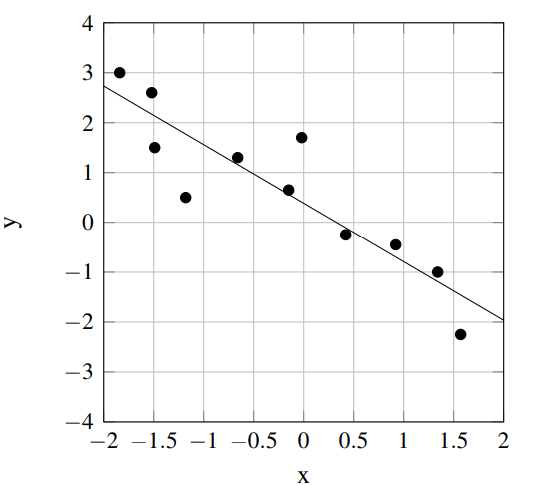
\includegraphics[scale=0.75]{img/linear-regression.png}
    \caption[Caption for LOF]{Primjer linearne regresije\footnotemark}
    \label{fig:linear-regression}
\end{figure}
\footnotetext{Preuzeto iz literature \citep{cupicML}.}

\begin{figure}[H]
    \centering
    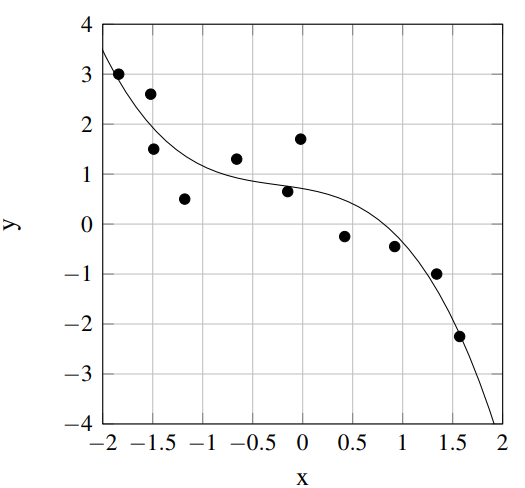
\includegraphics[scale=0.75]{img/polynom-regression.png}
    \caption[Caption for LOF]{Primjer polinomijalne regresije s kubnim polinomom\footnotemark}
    \label{fig:polynom-regression}
\end{figure}
\footnotetext{Preuzeto iz literature \citep{cupicML}.}

\subsection{Klasifikacija}
\label{chap:classification}
Klasifikacija \engl{Classification} je tehnika koja se koristi kada je određeni ulazni podatak potrebno smjestiti, odnosno klasificirati kao pripadnika određenog razreda. Izlazi tako organiziranog modela često poprimaju diskretne vrijednosti za razliku od regresije i takav model onda nazivamo klasifikator \engl{classifier}. Razlikujemo nekoliko različitih tipova klasifikatora:

\begin{enumerate}
    \item binarni klasifikator,
    \item višerazredni klasifikator i
    \item klasifikator više oznaka.
\end{enumerate}

\smallskip

Binarni klasifikator \engl{binary classifier} je tip klasifikatora koji zna odrediti pripada li ulazni podatak jednom od dva moguća razreda. Npr.\ sustav kao ulaze prima slike na kojima se nalazi ili mačka ili pas. Jednom naučeni klasifikator bi na temelju predane slike morao moći odrediti što se nalazi na slici, mačka ili pas. Naravno uz uvjet da se preda slika mačke ili psa.

Višerazredni klasifikator \engl{multi-class classifier} je tip klasifikatora koji zna odrediti pripada li ulazni podatak jednom od barem tri moguća razreda. Dakle, mora postojati minimalno tri različita razreda kako bi se klasifikator nazivao višerazrednim. U ovom radu ćemo se više fokusirati upravo na navedenom klasifikator koji će naučiti raspoznati tri moguća razreda, no o tome nešto kasnije.

Klasifikator više oznaka \engl{multi-label classifier} je tip klasifikatora koji predstavlja generalizaciju višerazrednog klasifikatora. Pogledajmo sljedeći primjer klasifikacije filmova za bolje razumijevanje. Pretpostavimo da film može imati sljedeće oznake: $(12+)$, $(16+)$ i $(18+)$ gdje svaka oznaka predstavlja minimalan broj godina kojih gledaoci filma moraju imati. Određivanje oznake za pojedini film je rezultat korištenja višerazrednog klasifikatora jer je potrebno odrediti pripada li film samo jednoj od navedene tri oznake. No što ako film poželimo klasificirati pomoću žanrova? Tada nam višerazredni klasifikator neće puno pomoći jer jedan film može imati više oznaka kao npr.\ "drama" i "komedija" i sl. U tom slučaju ćemo koristiti klasifikator više oznaka.

\bigskip

Klasifikaciju, kao i regresiju, možemo podijeliti na \textit{linearnu klasifikaciju} i \textit{nelinearnu klasifikaciju}, odnosno polinomijalnu.

Linearna klasifikacija \engl{linear classification} je tip klasifikacije u kojoj se granica između razreda aproksimira pomoću linearna krivulje, tj.\ pravca.

Nelinearna klasifikacija \engl{non-linear classification} je tip klasifikacije u kojoj se granica između razreda aproksimira pomoću nelinearne krivulje.

Ono što je zajedničko u oba slučaja je postojanje granice između razreda koja se u literaturi naziva \textit{decizijska granica} \citep{cupicANN}. O oblicima decizijskih granica će biti riječ kasnije.

Na slikama \ref{fig:linear-classification} i \ref{fig:non-linear-classification} su prikazani primjeri klasifikacija.

\begin{figure}[H]
    \centering
    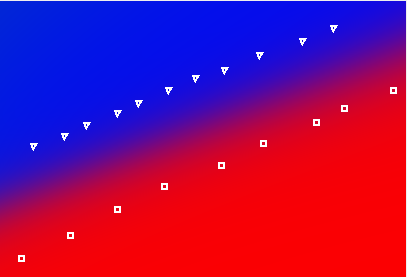
\includegraphics[scale=0.8]{img/linear-classification.png}
    \caption[Caption for LOF]{Primjer linearne klasifikacije\footnotemark}
    \label{fig:linear-classification}
\end{figure}
\footnotetext{Rezultat programske implementacije.}

\begin{figure}[H]
    \centering
    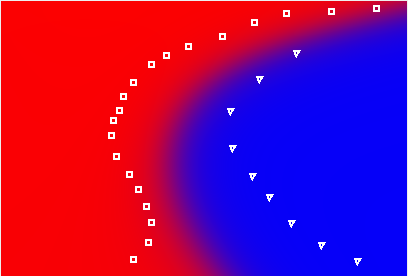
\includegraphics[scale=0.8]{img/non-linear-classification.png}
    \caption[Caption for LOF]{Primjer nelinearne klasifikacije\footnotemark}
    \label{fig:non-linear-classification}
\end{figure}
\footnotetext{Rezultat programske implementacije.}

\bigskip

\section{Algoritmi}
U području nadziranog učenja postoji veliki broj algoritama koji uvelike pridonose boljem učenju. Neki od poznatijih su:

\begin{itemize}
    \item Stroj potpornih vektora \engl{Support-vector machine, SVM},
    \item Stabla odluke \engl{Decision trees},
    \item Naivni Bayesov klasifikator \engl{Naive Bayes classifier},
    \item Slučajne šume \engl{Random forests},
    \item Algoritam k-najbližih susjeda \engl{K-nearest neighbors algorithm},
    \item Umjetna neuronska mreža \engl{Artificial neural network} i mnogi drugi.
\end{itemize}

\bigskip

Vidimo da postoji jako velika paleta algoritama od kojih su neki složeniji od drugih, neki daju bolje rezultate od drugih, no niti jedan od algoritama
nije u stanju uvijek dati najbolje rezultate za proizvoljan problem nadziranog učenja \citep{wiki:SUP}. Zbog navedenog vrijedi tzv.\ \textit{No free lunch} teorem koji nalaže da je za probleme koji zahtijevaju mnogo računalnih resursa poput pretraživanja prostora stanja i optimizacije parametara složenost\footnote{Često se ovako definirani problemi nazivaju \textit{NP}-teškim problemima \engl{Non-deterministic polynomial-time problems}.} u prosjeku jednaka za sve metode \citep{wiki:NFL}.

\bigskip
\bigskip

U sljedećem poglavlju ćemo se detaljnije baviti algoritmom \textit{umjetna neuronska mreža}. Pogledat ćemo kako je nastao koncept umjetnog neurona, strukturu umjetnog neurona, arhitekturu unaprijedne neuronske mreže te algoritam kojim unaprijedna neuronska mreža uči.

\chapter{Umjetne neuronske mreže}
U drugom poglavlju (\textit{Pregled područja}) dotaknuli smo se razlika između simboličke umjetne inteligencije i strojnog učenja i rekli smo kako simbolička umjetna inteligencija koristi simbolički pristup, tj.\ sve iskaze pokušava predočiti mnoštvom pravila pomoću ljudima čitljivim simbolima, dok se strojno učenje bavi raznim algoritmima pomoću kojih se računalni sustav uči. U ovom poglavlju bavit ćemo se algoritmom strojnog učenja koji koristi tzv.\ konektivistički pristup.

\section{Motivacija}
Ideja za konektivizmom \engl{connectivism} potaknuta je na temelju strukture ljudskog mozga te zbog izrazite brzine kojom mozak obrađuje podražaje. Danas je poznato da u ljudskom mozgu postoji oko 10\textsuperscript{11} neurona te 10\textsuperscript{15} međusobnih veza što znači da je svaki neuron u prosjeku povezan sa 10\textsuperscript{4} različitih veza \citep{cupicNENR}. To upravo dokazuje da mozak predstavlja jedan kompleksan i paralelan sustav zbog čega je konektivizam dobio ime te čemu algoritam umjetne neuronske mreže teži. Također, koncept ljudskog mozga nije uzet samo radi svoje izrazite brzine prilikom obrade podražaja, već i zbog činjenice da ga se može učiti na temelju velikog broja podataka koji su često ispunjeni raznim šumovima, što je realna situacija, te ga time potaknuti da razvije svojstvo generalizacije. Područje koje se bavi proučavanjem umjetnih neuronskih mreža naziva se neuro računarstvo \engl{neuro-computing} koje je jedno od grana mekog računarstva \engl{soft-computing}.

\section{Biološki neuron}
Neuroni \engl{neurons} su glavne stanice mozga i živčanog sustava. Zadaća im je da primaju podražaje iz okoline, da prenose određene akcije od mozga prema našim mišićima i da vode računa o pretvaranju električnog potencijala između pojedinih neurona u svim koracima procesa vođenja. Neuron je izgrađen od posebne strukture koja se sastoji od: \textit{tijela stanice} (ili češće \textit{soma}), \textit{dendrita}, \textit{aksona}, i \textit{sinapse}. Struktura biološkog neurona prikazana je na slici \ref{fig:bio-neuron}.

\begin{figure}[H]
    \centering
    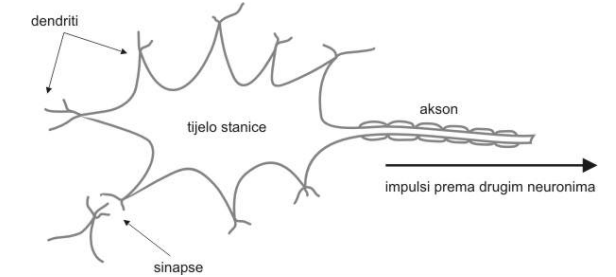
\includegraphics[scale=0.75]{img/bio-neuron.png}
    \caption[Caption for LOF]{Biološki neuron\footnotemark}
    \label{fig:bio-neuron}
\end{figure}
\footnotetext{Preuzeto iz literature \citep{cupicANN}.}

Dendriti \engl{dendrites} su ulazni dijelovi neurona, tj. strukture koje prihvaćaju impulse od drugih neurona preko veza koje se nazivaju sinapse. Suma svih ulaznih impulsa, tj.\ potencijala određuje hoće li dotični neuron biti aktiviran ili ne.

Aksoni \engl{axons} su izlazni dijelovi neurona, tj.\ strukture u kojima se generira određeni električni potencijal koji se dalje prosljeđuje sljedećem neuronu preko sinoptičkih veza.

Sinapse \engl{synapses} su, kao što je rečeno ranije, veze između dendrita jednog neurona i aksona drugog neurona \citep{bioNeuron}.

\section{Umjetni neuron}

\subsection{Povijesni pregled}

\subsubsection{MCP neuron}

\textbf{1943}.\ dva znanstvenika, Warren S. McCulloch i Walter H. Pitts, u svojem radu \textit{A Logical Calculus of Ideas Immanent in Nervous Activity} definiraju strukturu prvog umjetnog neurona koji se u literaturi često naziva kao \textit{MCP} neuron. Na slici \ref{fig:first-ai-neuron} prikazana je struktura MCP neurona. Dendriti su predstavljeni ulazima označenih slovima \textbf{E} od riječi ekscitacijski\footnote{ekscitacija - uzbuđenje ili aktivirano stanje zbog određenog podražaja (ekscitacija. Hrvatska enciklopedija, mrežno izdanje. Leksikografski zavod Miroslav Krleža, 2020. Pristupljeno 13. 5. 2020. <http://www.enciklopedija.hr/Natuknica.aspx?ID=17398>).} \engl{excitatory} te \textbf{I} od riječi inhibicijski\footnote{inhibicija - kočenje prijenosa živčanih impulsa (inhibicija. Hrvatska enciklopedija, mrežno izdanje. Leksikografski zavod Miroslav Krleža, 2020. Pristupljeno 13. 5. 2020. <http://www.enciklopedija.hr/Natuknica.aspx?ID=27450>).} \engl{inhibitory}, tijelo stanice je predstavljeno slovom \textbf{T} od riječi prag \engl{threshold} dok je akson predstavljen izlazom koji je označen slovom \textbf{Y} bez posebnog značenja.

Ekscitacijski ulazi uzrokuju da neuron postavne aktivan, tj.\ da se neuron "pali" \engl{fire}, dok inhibicijski ulazi uzrokuju da neuron postane neaktivan, tj.\ da se neuron "ne pali". Točnije, ako postoji barem jedan inhibicijski ulaz koji je aktivan, tada će neuron sigurno biti neaktivan neovisno o svim ostalim ulazima. Također, ako niti jedan od inhibicijskih ulaza nije aktivan, onda će neuron postati aktivan samo u slučaju kada je suma svih ekscitacijskih ulaza veća ili jednaka pragu, T \citep{McCullPits}. Matematički rečeno \citep{picton2000}:
\begin{equation}
\label{mcp:eq}
    Y = 
    \begin{cases}
        1, & \text{$\sum\limits_{i=1}^n I\textsubscript{i} = 0$ i $\sum\limits_{j=1}^m E\textsubscript{j} \geq T$} \\
        0, & \text{inače.}
    \end{cases}
\end{equation}

\begin{figure}[H]
    \centering
    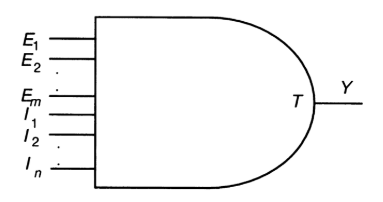
\includegraphics{img/first-ai-neuron.png}
    \caption[Caption for LOF]{MCP neuron\footnotemark}
    \label{fig:first-ai-neuron}
\end{figure}
\footnotetext{Preuzeto iz literature \citep{picton2000} iz poglavlja 1.4.2 Biologically inspired neural networks.}

MCP neuron mogao je modelirati osnovne Booleove logičke operacije kao što su operacija \textit{i} \engl{and}, operacija \textit{ili} \engl{or} i operacija negacije \engl{not} pa se može reći da neuron predstavlja logička vrata \engl{logic gate}, što je često korištena struktura prilikom konstrukcija uređaja poput računala koji mogu rješavati kompleksne logičke izraze. Shodno tomu se razvilo vjerovanje da se ljudski mozak sastoji upravo od mnoštva logičkih vrata, no nisu uzimali u obzir činjenicu da takva konstrukcija ne može biti učena te da nema svojstvo generalizacije \citep{picton2000}. 

Postoji još jedna bitna stavka oko strukture MCP neurona koja je prešutno korištena, a to su vrijednosti koje poprimaju ulazi i izlaz. Vrijednosti koje mogu poprimiti su iz skupa $\{0, 1\}$ i niti jedne druge, dok vrijednost praga može biti proizvoljan realan broj. To se implicitno moglo zaključiti iz spomenutih primjena na Booleove logičke operacije te iz formule \eqref{mcp:eq}.

\subsubsection{ADALINE}
\textbf{1960.}\ dva znanstvenika, Bernard Widrow i Marcian E. Hoff, u svojem radu \textit{Adaptive Switching Circuits} na temelju MCP neurona definiraju jednu od prvih neuronskih mreža nazvanu \textit{ADALINE} \engl{ADAptive LINear Elements}. Na slici \ref{fig:adaline-neuron} prikazana je struktura jednog neurona iz neuronske mreže ADALINE. Dendriti su predstavljeni ulazima označenim slovom \textbf{x}, tijelo stanice predstavljeno je težinama označenim slovom \textbf{w}, a akson je predstavljen izlazom označenim slovom \textbf{y}. Dakle, uočljivo je da postoje neke novine za razliku od MCP neurona. Ulogu ekscitacijskih, odnosno inhibicijskih ulaza sada imaju težine koje poprimaju vrijednosti iz skupa realnih brojeva, ulazi i izlaz poprimaju vrijednosti iz skupa $\{-1, 1\}$ i niti jedne druge, osim za ulaz \textbf{x\textsubscript{0}} čija je vrijednost uvijek 1, dok prag više nije eksplicitno zadan, već se u definiciju implicitno uključuje simbolom \textbf{w\textsubscript{0}} koji predstavlja konstantan pomak \engl{bias} \citep{picton2000}.

\begin{figure}[H]
    \centering
    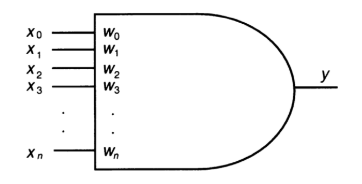
\includegraphics{img/adaline-neuron.png}
    \caption[Caption for LOF]{ADALINE neuron\footnotemark}
    \label{fig:adaline-neuron}
\end{figure}
\footnotetext{Preuzeto iz literature \citep{picton2000} iz poglavlja 1.4.2 Biologically inspired neural networks.}

Definiranje težina koje odgovaraju svaka svom ulazu revolucionarno je otkriće jer se time pokazalo da se tako definirani neuroni mogu učiti, što uvelike olakšava izvedbu računalnih sustava jer više nije potrebna kvantiteta da bi sustav funkcionirao, već kvalitetna izvedba. Umjesto praćenja koliko je ekscitacijskih, odnosno inhibicijskih ulaza aktivno, definirana je težinska suma \textit{net} koja je opisana sljedećom formulom:

\begin{equation}
    \label{net:eq}
    \text{$net = \sum\limits_{i=0}^n w\textsubscript{i} \cdot x\textsubscript{i}$}
\end{equation}

Vrijednost net-a je onda transformirana u izlaz \textbf{y} pomoću nelinearne funkcije koja pozitivne vrijednosti preslikava u 1, dok negativne vrijednosti ili vrijednosti koje su jednake 0 preslikava u -1. Matematička definicija dana je sljedećom formulom \citep{picton2000}:

\begin{equation}
\label{step:eq}
    y = 
    \begin{cases}
        +1, & \text{net $>0$} \\
        -1, & \text{net $\leq 0$}
    \end{cases}
\end{equation}

\bigskip

Koncept težina definiran je 1949.\ kada je Donald Hebb u svojem radu \textit{The Organization of Behavior: A Neuropsychological Theory} pokušao definirati da kada je akson neurona A dovoljno blizu da aktivira neuron B i to ponavlja veći broj puta, dolazi do metaboličkih promjena tako da se povećava efikasnost neurona A u aktiviranju neurona B \citep{hebb}. Često se navedeno pravilo naziva Hebbov princip učenja i može se definirati pomoću ADALINE neurona. Pravilo je dano sljedećom formulom \citep{picton2000}:

\begin{equation}
    \textit{w\textsubscript{i} = $\sum\limits_{p = 1}^P x\textsubscript{ip} \cdot y\textsubscript{p}$}
\end{equation}

Svaka težina \textit{w\textsubscript{i}} računa se kao težinska suma svih ulaza \textit{x\textsubscript{i}} sa željenim izlazom \textit{y} i to za svaki uzorak po skupu svih uzoraka koji su označeni slovom \textit{p}. Ako uzmemo u obzir da ulazi i izlazi poprimaju vrijednosti iz skupa $\{-1, 1\}$, onda je očito da iznos težine \textit{w\textsubscript{i}} raste ako su ulaz za tu težinu \textit{x\textsubscript{i}} i izlaz uzorka \textit{y\textsubscript{p}} aktivni, odnosno smanjuje ako su neaktivni. Iako se čini da je pravilo uspješno, pokazuje se da se njime ne uspijeva dobro naučiti mrežu jer se u izračun ne uzimaju stvarni izlazi neurona, već samo oni željeni izlazi.

Zbog navedenog nedostatka Hebbovog principa, Widrow i Hoff su došli do ideje da bi se težine morale ažurirati pomoću pogreške \engl{error} koja se događa između željenog izlaza i stvarnog izlaza te algoritma gradijentni spust. Navedeni princip nazvan je: \textit{delta pravilo} \engl{the delta rule} ili Widrow-Hoffovo pravilo, a danas je poznato i pod nazivom: pravilo najmanjeg srednjeg kvadrata \engl{least mean square rule, LMS}. Time su uspjeli postići da mreža ADALINE pokazuje jako dobre rezultate tijekom procesa učenja, a to se implicitno potkrepljuje riječju \textit{ADAptive} iz imena što znači prilagodljiv \citep{picton2000}. Detaljnije definicije i izvode formula pokazat ćemo u poglavlju gdje se govori o učenju unaprijedne neuronske mreže algoritmom propagacije pogreške unatrag.

Glavni nedostatak ADALINE neuronske mreže je činjenica da se njome uređaji konstruiraju isključivo fizičkim putem što je puno puta nepraktično i skupo za projektirati. U narednim poglavljima reći ćemo nešto o drugačijem izvodu umjetnih neuronskih mreža pomoću računalnih programa koje je puno lakše uklopiti u električne uređaje.

\subsection{Perceptron}
\textbf{1958.}\ znanstvenik Frank Rosenblatt u svojem radu \textit{The perceptron: a probabilistic model for information storage and organization in the brain} na temelju MCP neurona i Hebbovog principa učenja definira strukturu, perceptron\footnote{Dolazi od latinske riječi \textit{percepcio} što u prijevodu znači razumjeti \engl{understand}.}, čija je glavna ideja da se računalnim programom pokuša konstruirati sustav koji će moći učiti na temelju danih podražaja, dakle iz iskustva. U to vrijeme je ta ideja bila suluda i izazvala je mnoge kontroverze među pionirima umjetne inteligencije. The New York Times, dnevne američke novine, te iste godine opisuju perceptron kao zametak \engl{embryo} računala koji, jednom kada se kreira i usavrši, bi predstavljao prvi računalni sustav koji bi bio u stanju opažati, prepoznati i identificirati svoju okolinu bez ljudskog osposobljavanja ili kontrole.\footnote{The New York Times, \textit{Electronic 'Brain' Teaches Itself}, stranica 9, srpanj 13, 1958.}

\begin{figure}[H]
    \centering
    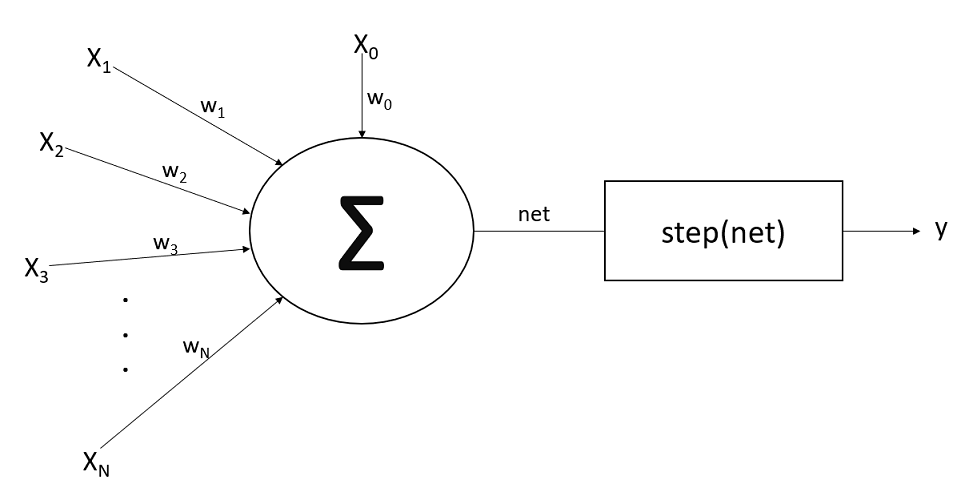
\includegraphics[scale=0.5]{img/step-neuron.png}
    \caption[Caption for LOF]{Umjetni neuron perceptrona\footnotemark}
    \label{fig:step-neuron}
\end{figure}
\footnotetext{Izrađeno pomoću powerpoint-a i na temelju modela umjetnog neurona iz literature \citep{cupicANN}.}

Struktura perceptrona je, kao što je rečeno ranije, motivirana strukturom MCP neurona. Na slici \ref{fig:step-neuron} nalazi se prikaz perceptrona koji je predstavljen kao generalizirani MCP neuron gdje je uloga ekscitacijskih, odnosno inhibicijskih ulaza zamijenjena težinama slično kao i kod ADALINE neurona. Novost u strukturi je prikaz funkcije skoka \engl{step} koja je implicitno postojala i kod izvornog MCP neurona, no ovdje je navedena eksplicitno jer se takav oblik koristi u literaturi. Također, ovakva struktura se u literaturi često naziva jednoslojni perceptron \engl{single-layer perceptron}, a kasnije ćemo se susresti i s višeslojnim perceptronom \engl{multi-layered perceptron}.

Glavna zamisao koju je Rosenblatt dokumentirao u svom radu bila je izvesti nekakvu vrstu binarnog klasifikatora\footnote{Vidi \ref{chap:classification} Klasifikacija.} i definirati algoritam kojim bi se taj isti klasifikator uspio naučiti \citep{rosenblatt}. Ideja algoritma je da se težine ažuriraju pomoću pogreške koja se događa između željenog izlaza i stvarnog izlaza te se onda pomnoži sa nekom konstantom koju ćemo definirati u nastavku. Pravilo učenja perceptrona dano je algoritmom \ref{algo:alg-perceptron}.

\begin{algorithm}
\caption{Pravilo učenja perceptrona\footnotemark}
\label{algo:alg-perceptron}
    \begin{enumerate}
        \item[\textbf{1.}] Ciklički prolazi kroz svih \textit{N} uzoraka za učenje, jedan po jedan.
        \item[\textbf{2.}] Klasificiraj trenutni uzorak.
        \begin{enumerate}
            \item[\textbf{1.}] Ako se klasificira korektno, ne mijenjaj težine i
            \begin{enumerate}
                \item[\textbf{1.}] ako je to \textit{N}-ti uzastopni uzorak klasificiran korektno, prekini učenje,
                \item[\textbf{2.}] inače prijeđi na sljedeći uzorak.
            \end{enumerate}
            \item[\textbf{2.}] Ako se ne klasificira korektno, korigiraj težine perceptrona prema sljedećem izrazu: 
            \begin{equation}
            \label{percep:eq}
                w\textsubscript{i}(k+1) \leftarrow w\textsubscript{i}(k) + \eta \cdot (d-y) \cdot x\textsubscript{i}
            \end{equation}
        \end{enumerate}
    \end{enumerate}
\end{algorithm}
\footnotetext{Iz literature \citep{cupicANN}.}

U procesu učenja klasifikatora može se uočiti da su spomenuti samo uzorci za učenje, no sada znamo i da postoji još nekoliko mehanizama koji uvelike doprinose da klasifikator razvije svojstvo generalizacije. Neki od tih mehanizama su npr.\ uporaba skupa za provjeru i skupa za testiranje, ali navedenim algoritmom smo htjeli pokazati elementarni proces učenja pa se time ovdje nismo htjeli zamarati. Ono što nas najviše zanima je interpretacija formule \eqref{percep:eq}. Index \textit{i} predstavlja \textit{i}-tu vrijednost, tj.\ \textit{w\textsubscript{i}} je \textit{i}-ta težina za \textit{i}-ti ulaz, što se može vidjeti i na slici \ref{fig:step-neuron}, \textit{k} je \textit{k}-ta iteracija procesa učenja, \textit{d} predstavlja željeni \engl{desired} izlaz neurona, dok \textit{y} predstavlja stvarni izlaz neurona te $\eta$ (eta) predstavlja parametar koji se zove stopa učenja \engl{learning rule}. To je pozitivan realan broj malog iznosa (najčešće između 0.001 i 0.5) kojim se regulira kolikom mjerom će se ažurirati trenutna težina neurona. Ako je $\eta$ jako mali broj, onda će proces učenja biti prespor, tj.\ težine će se mizerno malo ažurirati. Ako je $\eta$ jako veliki broj, onda će proces učenja zasigurno divergirati jer će se težine ažurirati povećim brojevima i vrijednosti će "eksplodirati". Navedeni parametar ima jako bitnu ulogu prilikom optimizacije raznih \textit{NP} teških problema koji koriste inačice algoritma gradijentni spust o kojemu će biti nešto riječi kasnije kada se dotaknemo algoritma propagacije pogreške unatrag.

\bigskip

Dakle, Rosenblatt je uspješno uspio iznijeti svoje teze iako su mnogi sumnjali u njih. No, mreže koje su etiketirane kao jednoslojni perceptron imaju jednu veliku manu kao i prethodno navedene ADALINE neuronske mreže, a to je činjenica da uspješno djeluju samo kada je problem linearno interpretabilan, tj.\ kada su izlazi dotičnih neuronskih mreža linearno odvojivi \engl{linearly separable}, a ADALINE neuronska mreža to još dodatno potvrđuje i imenom \textit{LINear Elements}. Ako se kratko vratimo na poglavlje u kojem smo govorili o tipovima klasifikacija, onda možemo vidjeti da smo problem klasifikacije podijelili na linearnu i nelinearnu klasifikaciju. Jednoslojni perceptroni su tipovi linearnih klasifikatora što znači da bi problem na slici \ref{fig:linear-classification} uspješno uspjeli klasificirati, dok problem na slici \ref{fig:non-linear-classification} ne bi jer se radi o nelinearnoj klasifikaciji. Primjeri koji se često vežu uz jednoslojne perceptrone jesu osnovne Booleove logičke operacije i, ili i negacija. Svaka od njih ima linearno interpretabilan izlaz te ih je bilo moguće realizirati. U to vrijeme je to bilo značajno otkriće kao što je i spomenuto kod opisa primjene ADALINE neuronskih mreža. S druge strane, npr.\ operacija isključivo ili (XOR) nema linearno interpretabilan izlaz te se ne može realizirati jednoslojnim perceptronom kao takvim, već se mora konstruirati dvoslojni perceptron kako bi realizacija bila korektna. \footnote{Zanimljivi primjeri mogu se pronaći u skripti Umjetne neuronske mreže \citep{cupicANN}.} No, ideja o višeslojnom perceptronu je tada bila tek u procesu stvaranja jer pravilo učenja perceptrona koje je predložio Rosenblatt je djelovalo samo na jednoslojne perceptrone. 1969.\ Marvin L. Minsky i Seymour A. Papert u svojem radu \textit{Perceptrons} jasno iznose nedostatke perceptrona koji je Rosenblatt definirao i to ponajviše o nemogućnostima rješavanja nelinearno odvojivih problema i učenja višeslojnih perceptrona. Time je i započela prva zima u eri umjetne inteligencije \engl{1st AI winter} kada se konektivistički pristup zamjenjuje simboličkim. Konektivizam će biti po strani sve negdje do 1986.\ kada će se po prvi put definirati algoritam kojim će višeslojni perceptron moći učiti, a to je algoritam propagacije pogreške unatrag.

\section{Općenito o umjetnim neuronskim mrežama}
Do sada smo se upoznali s modelom umjetnog neurona i prvim modelima neuronskih mreža, ADALINE i perceptron i vidjeli smo nedostatke koji isti sadrže. Mali broj neurona može davati dosta uspješne rezultate, no ograničeni su na jako jednostavne i  specifične probleme kao npr.\ konstrukcija jednostavnih Booleovih logičkih operacija što smo spomenuli ranije. Ljudski mozak je evidentno puno kompleksniji od strukture par neurona te se time došlo na ideju povezati veliki broj neurona u jednu veliku strukturu, tj.\ algoritam koji će biti vjerni prikaz ljudskog mozga, a takav algoritam je nazvan umjetna neuronska mreža. Na slici \ref{fig:ann} je prikazana tipična građa jedne unaprijedne višeslojne potpuno povezane umjetne neuronske mreže.

\begin{figure}[H]
    \centering
    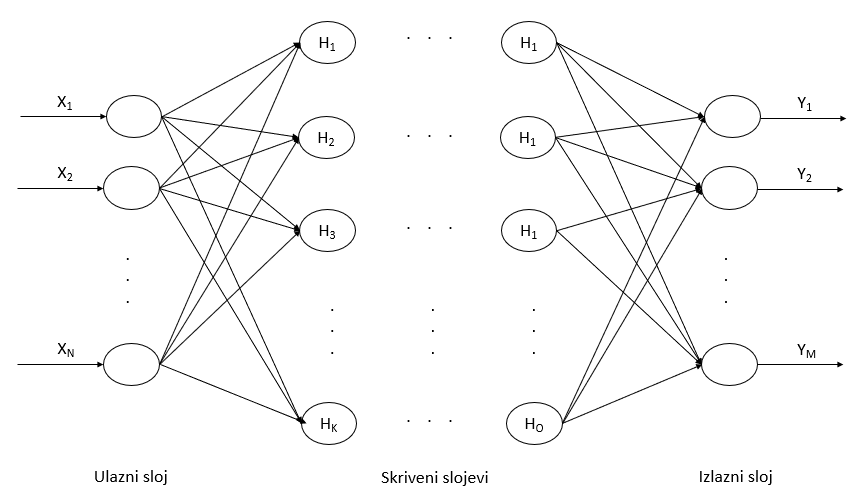
\includegraphics[scale=0.6]{img/ann.png}
    \caption[Caption for LOF]{Tipična građa umjetne neuronske mreže\footnotemark}
    \label{fig:ann}
\end{figure}
\footnotetext{Izrađeno pomoću powerpoint-a i na temelju modela umjetne neuronske mreže iz literature \citep{cupicNENR}.}

Dakle, mreža se sastoji od tri različite vrste slojeva: ulazni, skriveni i izlazni sloj. Ulazni sloj je sloj na koji se dovode uzorci za koje želimo da mreža nešto napravi i prikazani su slovom \textbf{x}. Izlazni sloj je sloj na kojemu će se nalaziti izlazi za navedeni uzorak u ulaznom sloju i prikazani su slovom \textbf{y}. Skriveni sloj je sloj koji jedini nije vidljiv izvana i u kojemu se sva logika umjetne neuronske mreže događa. Neuroni skrivenog sloja označeni su slovom \textbf{h} i broj slojeva koji se nalaze u skrivenom sloju može biti proizvoljan. Primijetite koji se indeksi koriste kod enumeracije svakog od slojeva. U ulaznom sloju neuronska mreža očekuje \textit{n} ulaza, u izlaznom sloju se očekuje \textit{m} izlaza, dok u skrivenom sloju broj neurona može varirati po sloju, stoga su korišteni proizvoljni indeksi označeni slovima \textit{k} i \textit{o}.

U navedenoj strukturi pretpostavili smo da je svaki neuron nekog sloja povezan sa svakim neuronom njemu sljedećeg sloja i to samo tog sloja, osim izlaznog sloja koji je posljednji sloj neuronske mreže. Takve mreže ćemo nazivati slojevitim potpuno povezanim mrežama i njihova je zadaća da za neki fiksan ulaz generiraju neki stabilan izlaz \citep{cupicNENR}. U matematičkom smislu, navedena operacija naziva se preslikavanje i to je glavna tema ovog rada kojoj ćemo se uskoro posvetiti detaljnije. Međutim, postoje i različite vrste mreža koje ne moraju biti niti slojevite niti potpuno povezane, a mogu imati i cikluse. Kod takvih mreža neuroni mogu biti povezani i s neuronima prethodnog sloja te se time postiže da neuronske mreže budu promjenjive kroz vrijeme i da imaju mogućnost čuvanja nekog određenog stanja, tj.\ možemo reći da razvijaju nekakvu vrstu memorije. Na slici \ref{fig:cyclic-ann} je prikazana struktura jedne cikličke umjetne neuronske mreže koja je gotovo identična neuronskoj mreži na slici \ref{fig:ann}, no dodana je jedna povratna veza kojom se cijela ideja mreže mijenja.

\begin{figure}[H]
    \centering
    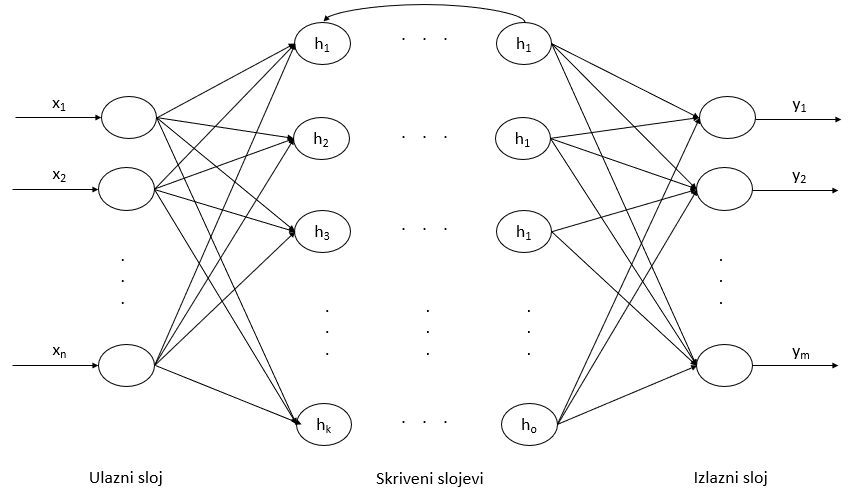
\includegraphics[scale=0.6]{img/cycle-ann.png}
    \caption[Caption for LOF]{Tipična građa cikličke umjetne neuronske mreže\footnotemark}
    \label{fig:cyclic-ann}
\end{figure}
\footnotetext{Izrađeno pomoću powerpoint-a i na temelju modela umjetne neuronske mreže iz literature \citep{cupicANN}.}

Često spominjemo sintagme poput struktura ili građa umjetne neuronske mreže, no u raznim literaturama koristi se sintagma arhitektura umjetne neuronske mreže pa ćemo i mi ubuduće koristiti upravo takav opis. Arhitektura umjetne neuronske mreže definira se na sljedeći način: uvijek započinje brojem neurona ulaznog sloja, zatim se definiraju skriveni slojevi i to svaki sloj je predstavljen brojem neurona tog sloja i na kraju se nalazi broj neurona izlaznog sloja. Npr.\ jedna od arhitektura mogla bi biti 2x5x4x3 i nju tumačimo na sljedeći način: mreža se sastoji od četiri sloja; ulaznog, dva skrivena i izlaznog. Ulazni sloj je sastavljen od 2 neurona, prvi skriveni sloj je sastavljen od 5 neurona, drugi skriveni sloj je sastavljen od 4 neurona i izlazni sloj je sastavljen od 3 neurona. Shodno navedenom bi npr.\ jednu inačicu Rosenblattovog perceptrona mogli definirati kao 3x1 jer on ne sadrži niti jedan skriveni sloj. Kasnije ćemo pogledati na koji način različite arhitekture utječu na uspješnost jedne unaprijedne neuronske mreže tijekom učenja klasifikatora.

\section{Unaprijedna neuronska mreža}
Najčešće korišteni tip umjetne neuronske mreže je unaprijedna višeslojna potpuno povezana umjetna neuronska mreža \engl{feedforward multilayered fully connected artificial neural network} čiju smo generalnu arhitekturu već upoznali na slici \ref{fig:ann}. Često se ista u literaturi naziva i samo unaprijedna neuronska mreža zbog lakšeg dokumentiranja rada pa ćemo i mi preuzeti tu konvenciju, a implicitno ćemo biti svjesni punog imena i svojstva. Također, unaprijedna neuronska mreža je pravi primjer višeslojnog perceptrona jer se očigledno sastoji od više slojeva te se može učiti danas već nekolicinom uspješnih algoritama.

Glavna zadaća unaprijedne neuronske mreže, kao što i samo ime nalaže, je da ulaze propagira kroz sve slojeve sve do izlaznog pri čemu se izvršava operacija mapiranja između ulaza i izlaza mreže na mnoštvo različitih načina. Također, sve operacije koje ćemo susresti se vrlo efikasno mogu prikazati matričnim računima čime se računalna izvedba implementacije i učenja unaprijedne neuronske mreže čini jako jednostavnim, no ponekad ipak to neće biti slučaj jer postoji nekolicina parametara koje je potrebno "nariktati" različitim metoda koje često i nisu zahvalne.

Pogledajmo jednu jednostavnu unaprijednu neuronsku mrežu s arhitekturom 2x3x2 na slici \ref{fig:ffann}.
Crnom bojom su označeni ulazi u ulaznom sloju, plavom bojom su označene težine između dva neurona, zelenom bojom je označen bias, a crvenom bojom su označeni izlazi iz neurona pa krenimo redom s notacijama:

\begin{description}
\item[\textcolor{myblue}{w\textsubscript{jk}\textsuperscript{(l)}} :] težina između k-tog neurona (l--1)-vog sloja i j-tog neurona l-tog sloja.
\item[\textcolor{mygreen}{b\textsubscript{j}\textsuperscript{(l)}} :] bias j-tog neurona l-tog sloja.
\item[\textcolor{red}{y\textsubscript{j}\textsuperscript{(l)}} :] izlaz j-tog neurona l-tog sloja.
\end{description}

\begin{figure}[H]
    \centering
    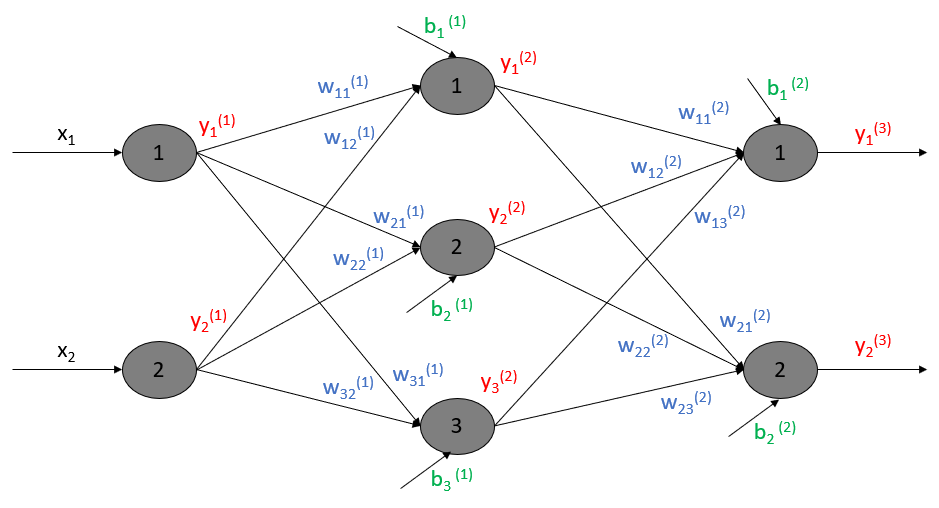
\includegraphics[scale=0.55]{img/ffann.png}
    \caption[Caption for LOF]{2x3x2 arhitektura unaprijedne neuronske mreže\footnotemark}
    \label{fig:ffann}
\end{figure}
\footnotetext{Izrađeno pomoću powerpoint-a i na temelju modela umjetne neuronske mreže iz literature \citep{nielsenANN}.}

Prije nego se dotaknemo matematičke podloge, definirajmo ponovno strukturu umjetnog neurona.

Do ovog trenutka upoznali smo se samo s dvije vrste neurona, a to su MCP neuron koji se koristio u Rosenblattovu modelu perceptron i ADALINE neuron. Pokazali smo i da se tako definirani neuroni koriste samo kada je problem kojeg rješavamo linearno interpretabilan. To se događa zbog funkcije skoka koja se nalazi na izlazu neurona te zbog nje učenje višeslojnog perceptrona nije moguće jer funkcija skoka nije derivabilna te algoritam propagacije pogreške unatrag neće biti moguće provesti, ali o tome ćemo reći nešto detaljnije kada se dotaknemo učenja unaprijedne neuronske mreže. Zbog navedenog ćemo uvesti jednu generalnu strukturu umjetnog neurona koji ne mora koristiti funkciju skoka kao funkciju izlaza. Na slici \ref{fig:ai-neuron} nalazi se ažurirana struktura umjetnog neurona. Vidimo da je struktura gotovo identična već spomenutom neuronu na slici \ref{fig:step-neuron} osim oznake za funkciju na izlazu. Funkcije koje se nalaze na izlazu neurona nazivaju se aktivacijske funkcije\footnote{U starijim literaturama češći naziv bio je prijenosna funkcija.} i njihova je zadaća, kao što i samo ime nalaže, aktiviranje, odnosno deaktiviranje neurona ovisno o svojstvima funkcije i vrijednosti argumenta funkcije, tj.\ net vrijednosti i takvu funkciju ćemo označavati sa slovom \textbf{g}.\footnote{Općenito, svaki neuron može ima svoju aktivacijsku funkciju te zbog toga bi ih trebali indeksirati, ali zbog jednostavnosti ćemo ih sve označavati samo s g.} Dakle, MCP neuron kojeg smo nedavno obrađivali kao aktivacijsku funkciju koristi funkciju skoka. U narednom poglavlju ćemo dati pregled često korištenih aktivacijskih funkcija te njihovih formula kao i derivacija istih, no u ovom trenutku je jedino bitno da smo svjesni da one postoje radi matričnog prikaza unaprijedne neuronske mreže.

\begin{figure}[H]
    \centering
    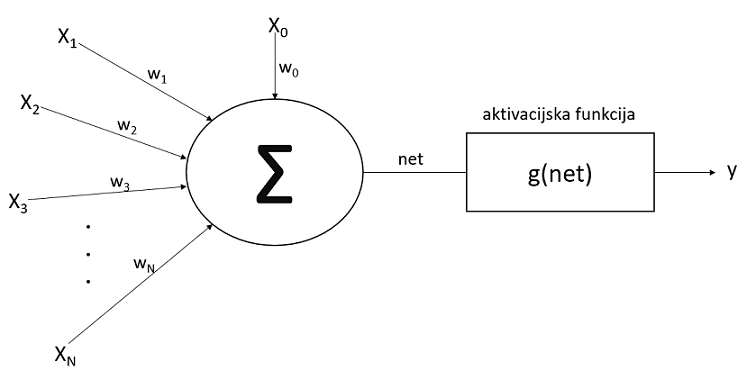
\includegraphics[scale=0.6]{img/ai-neuron.png}
    \caption[Caption for LOF]{Umjetni neuron\footnotemark}
    \label{fig:ai-neuron}
\end{figure}
\footnotetext{Izrađeno pomoću powerpoint-a i na temelju modela umjetnog neurona iz literature \citep{cupicANN}.}

\bigskip

Prisjetimo se formule za izračun net vrijednosti koju smo definirali kada smo pričali o ADALINE neuronu \eqref{net:eq}:
\[\text{$net = \sum\limits_{i=0}^n w\textsubscript{i} \cdot x\textsubscript{i}$}\]
Primijetite da sumacija u ovom slučaju ide od 0 jer, ako se prisjetite strukture ADALINE neurona, postoji težina w\textsubscript{0} koja predstavlja bias i ulaz x\textsubscript{0} konstante vrijednosti koja iznosi 1. Na slici \ref{fig:ffann} bias pojedinog neurona je eksplicitno naveden slovom \textbf{b} te zbog efikasnosti prikaza je izostavljen konstantni ulaz. S obzirom na to da se ADALINE neuron jedino mogao nalaziti u jednoslojnoj neuronskoj mreži, korišteno je slovo \textbf{x} kao ulaz neurona, a u našem slučaju mreža je višeslojna pa ćemo ulaze svih slojeva osim ulaznog notirati slovom \textbf{y}. Ako se pitate zašto je tomu tako, onda se dobro pitate jer je ta činjenica prešućena. Naime, ideja samog ulaznog sloja je da prenese dane ulaze na izlaz neurona te će tako izlazi ulaznog sloja biti jednaki ulazima, odnosno ne postoji nikakvo računanje net vrijednosti jer težine nisu prisutne. Također, svaki neuron osim ulaznih sadrži svoju net vrijednost. Uzevši u obzir navedene promjene i navedene notacije, net vrijednost pojedinog neurona možemo definirati na sljedeći način:

\begin{equation}
    \label{eq:novi-net}
    \text{$net\textsubscript{j}\textsuperscript{(l+1)} = \sum\limits_{k=1}^n w\textsubscript{j}\textsubscript{k}\textsuperscript{(l)} \cdot y\textsubscript{k}\textsuperscript{(l)} + b\textsubscript{j}\textsuperscript{(l)}$}
\end{equation}

gdje net\textsubscript{j}\textsuperscript{(l)} predstavlja net vrijednost j-tog neurona l-tog sloja pri čemu \textit{l} predstavlja sloj koji nije ulazni, a sumacija se proteže do \textit{n} pri čemu \textit{n} predstavlja broj neurona u (l--1)-vom sloju. Nakon izračuna, net vrijednost je potrebno "provući" kroz aktivacijsku funkciju kako bi se dobio izlaz za dotični neuron. Izračun za izlaz dan je sljedećom formulom: 

\begin{equation}
    \label{eq:izlaz}
    \text{$y\textsubscript{j}\textsuperscript{(l+1)} = g(net\textsubscript{j}\textsuperscript{(l+1)}) = g(\sum\limits_{k=1}^n w\textsubscript{j}\textsubscript{k}\textsuperscript{(l)} \cdot y\textsubscript{k}\textsuperscript{(l)} + b\textsubscript{j}\textsuperscript{(l)})$}
\end{equation}

Evidentno je da se formula može zapisati i matrično po svakom sloju neuronske mreže izuzev ulaznog. Uvedimo još nekoliko notacija:

\begin{description}
\item[W\textsuperscript{(l)} :] matrica svih težina l-tog sloja gdje su retci težine iz svih neurona (l--1)-vog sloja u jedan neuron l-tog sloja.
\item[$\Vec{b}\textsuperscript{ (l)}$ :] vektor svih bias vrijednosti l-tog sloja.
\item[$\Vec{net}\textsuperscript{(l)}$ :] vektor svih net vrijednosti l-tog sloja.
\item[$\Vec{y}\textsuperscript{ (l)}$ :] vektor svih izlaza l-tog sloja.
\end{description}

Nakon uvedenih notacija, formule možemo prikazati na sljedeći način:

\begin{equation}
    \label{eq:net-matrice}
    \text{$\Vec{net}\textsuperscript{(l+1)} = \textbf{W}\textsuperscript{(l)} \cdot \Vec{y}\textsuperscript{ (l)} + \Vec{b}\textsuperscript{ (l)}$}
\end{equation}

\begin{equation}
    \label{eq:izlaz-matrice}
    \text{$\Vec{y}\textsuperscript{ (l+1)} = g(\Vec{net}\textsuperscript{(l+1)}) = g(\textbf{W}\textsuperscript{(l)} \cdot \Vec{y}\textsuperscript{ (l)} + \Vec{b}\textsuperscript{ (l)})$}
\end{equation}

Radi lakšeg razumijevanja, pokušajmo pokazati kako će izgledati matrica težina, vektor bias-a i vektor izlaza ako promatramo vezu između prvog i drugog sloja, odnosno ulaznog i skrivenog sa slike \ref{fig:ffann}.

\[
  \textbf{W\textsuperscript{ (1)}} =
  \begin{bmatrix}
    w\textsubscript{11}\textsuperscript{(1)} & w\textsubscript{12}\textsuperscript{(1)}\\
    w\textsubscript{21}\textsuperscript{(1)} & w\textsubscript{22}\textsuperscript{(1)}\\
    w\textsubscript{31}\textsuperscript{(1)} & w\textsubscript{32}\textsuperscript{(1)}
  \end{bmatrix},\quad
  \vec{y}\textsuperscript{ (1)} = 
  \begin{bmatrix}
   y\textsubscript{1}\textsuperscript{(1)} \\
   y\textsubscript{2}\textsuperscript{(1)}
  \end{bmatrix},\quad
  \vec{b}\textsuperscript{ (1)} = 
  \begin{bmatrix}
    b\textsubscript{1}\textsuperscript{(1)} \\
    b\textsubscript{2}\textsuperscript{(1)} \\
    b\textsubscript{3}\textsuperscript{(1)}
  \end{bmatrix}
\]

Vidimo da dimenzije svih matrica odgovaraju za operaciju produkta matrica, odnosno operaciju zbroja matrica. Isti postupak ponavljamo za svaki sloj unaprijedne neuronske mreže sve dok ne dobijemo izlaze izlaznog sloja kada stajemo s računom pri čemu još jednom valja naglasiti da izlazi jednog sloja postaju ulazi onom sljedećem.

\subsection{Aktivacijske funkcije}
Aktivacijska funkcija \engl{activation function}, kao što smo i spomenuli kod računa unaprijedne neuronske mreže, je funkcija koja se nalazi tik prije izlaza neurona i određuje hoće li dotični biti aktiviran, odnosno deaktiviran, tj.\ hoće li se "paliti" ili ne. Danas postoji veliki broj aktivacijskih funkcija, no mi ćemo spomenuti one koje se najviše koriste i koje su korištene u ovom radu, a u poglavlju s rezultatima ćemo pokazati kako neke od njih utječu na sam izgled decizijske granice.

\subsubsection{Binarna funkcija skoka}
Binarna funkcija skoka \engl{binary step function} je funkcija koja se temelji na nekom fiksnom pragu i s njome smo se susreli kod MCP neurona i Rosenblattovog perceptrona. Neuroni koji koriste ovu kao aktivacijsku funkciju nazivaju se TLU \engl{threshold logic unit} neuroni. Na slici \ref{fig:step-fun} nalazi se graf jedne takve funkcije. Nedostatak ovakve funkcije kod učenja višeslojnog perceptrona je što nije derivabilna i što koristi binarne izlaze pa višerazredna klasifikacija nije moguća. 

\begin{figure}[H]
    \centering
    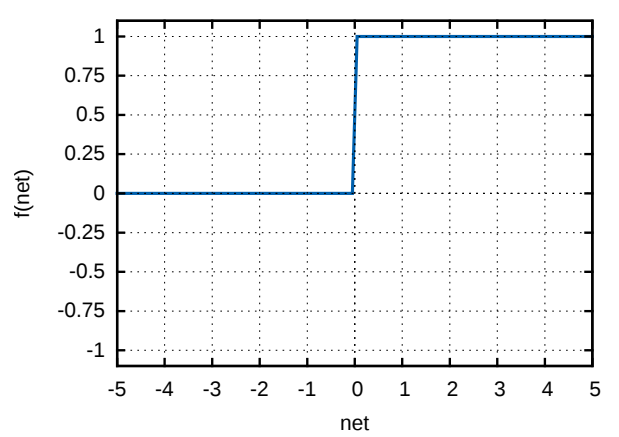
\includegraphics[scale=0.5]{img/step-fun.png}
    \caption[Caption for LOF]{Funkcija skoka \textit{f(net) = step(net)}\footnotemark}
    \label{fig:step-fun}
\end{figure}
\footnotetext{Preuzeto iz literature \citep{cupicANN}.}

\subsubsection{Linearne aktivacijske funkcije}
Linearne aktivacijske funkcije su funkcije oblika \textit{y = ax + b} i one generiraju izlaz koji je proporcionalan ulazu pa su zbog toga nešto efikasnije od funkcije skoka. No, i one imaju dosta nezgodne nedostatke kada govorimo o učenju višeslojnog perceptrona. One jesu derivabilne, ali njihova derivacija je konstanta što za algoritam propagacije pogreške unatrag nikako nije dobro. Također, ako svaki sloj koristi linearnu aktivacijsku funkciju, onda ne postoji nikakva razlika među slojevima jer će na izlazu opet biti linearna funkcija zbog pravila o linearnosti koji kaže da je linearna kombinacija linearnih funkcija također linearna funkcija. Posljedica toga je da linearna aktivacijska funkciju višeslojni perceptron pretvara u jednoslojni te se tada radi o običnom problemu linearne regresije. Na slici \ref{fig:id-fun} nalazi se graf jedne takve funkcije.

\begin{figure}[H]
    \centering
    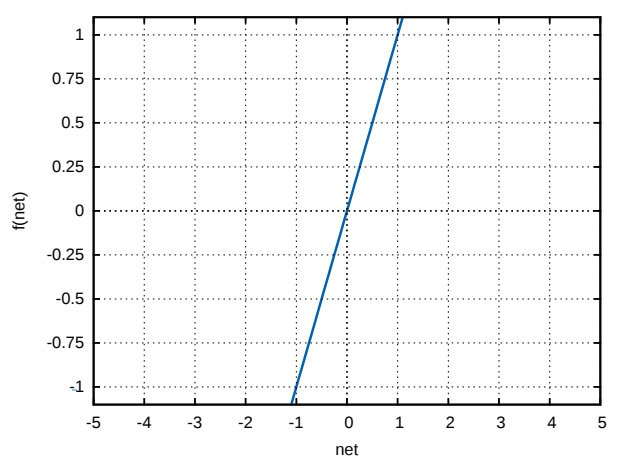
\includegraphics[scale=0.5]{img/id-fun.png}
    \caption[Caption for LOF]{Funkcija identiteta \textit{f(net) = net}\footnotemark}
    \label{fig:id-fun}
\end{figure}
\footnotetext{Preuzeto iz literature \citep{cupicANN}.}

\subsubsection{Nelinearne aktivacijske funkcije}
Nelinearne aktivacijske funkcije su najčešće korištene funkcije kada se radi o učenju višeslojnog perceptrona jer uvelike čine unaprijednu neuronsku mrežu ekspresivnijom i ostavljaju mogućnost kreiranja jako dubokih neuronskih mreža po broju skrivenih slojeva. Većina njih je derivabilna što znači da se mogu koristiti u učenju algoritmom propagacije pogreške unatrag te njihove derivacije se mogu zapisati pomoću samih funkcija što znatno olakšava i implementaciju istih.

\begin{enumerate}
    \item \textbf{Sigmoidalna/logistička funkcija} (prikazana na slici \ref{fig:sigm-fun}):
    \begin{equation}
        \label{eq:sigm}
        sigm(net) = \frac{1}{1 + e^{-net}},
    \end{equation}
    \begin{equation}
        \label{eq:sigm-der}
        sigm'(net) = sigm(net) \cdot (1 - sigm(net)).
    \end{equation}
    Izlaze mapira na vrijednosti iz intervala $(0, 1)$. Kod ove funkcije se javlja problem iščezavajućeg gradijenta \engl{vanishing gradient} što znači da će jako velike ulaze, odnosno jako male izlaze mapirati na vrijednosti oko 1, odnosno oko 0 i time će se učenje mreže znatno usporiti jer će ažuriranje težina gotovo pa stagnirati. Još jedan problem koji se javlja je centriranje svih izlaza oko vrijednosti 0.5, a ne oko 0. To se pokazuje dosta lošim svojstvom kroz literature. Neuroni koji koriste sigmoidalnu funkciju kao aktivacijsku nazivaju se sigmoidalni neuroni. Također, izvođenje ove funkcije je računalno skupo i danas se slabo više koristi.
    \begin{figure}[H]
        \centering
        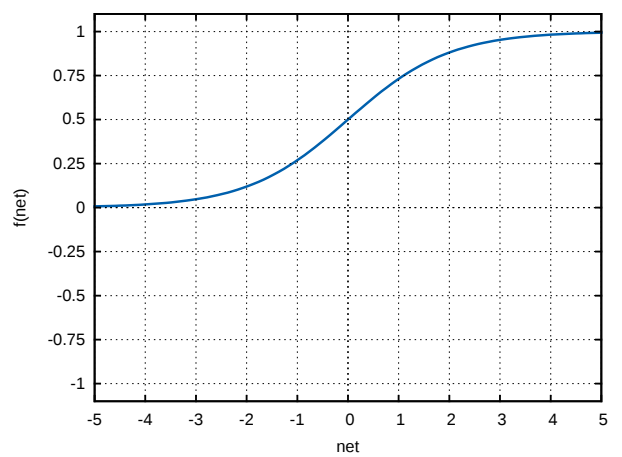
\includegraphics[scale=0.5]{img/sigm-fun.png}
        \caption[Caption for LOF]{Sigmoidalna funkcija \textit{f(net) = sigm(net)}\footnotemark}
        \label{fig:sigm-fun}
    \end{figure}
    \footnotetext{Preuzeto iz literature \citep{cupicANN}.}
    \item \textbf{Funkcija tangens hiperbolni} (prikazana na slici \ref{fig:tanh-fun}):
    \begin{equation}
        \label{eq:tanh}
        tanh(net) = \frac{e^{net} - e^{-net}}{e^{net} + e^{-net}} = 2 \cdot sigm(2 \cdot net) - 1,
    \end{equation}
    \begin{equation}
        \label{eq:tanh-der}
        tanh'(net) = 1 - tanh^2(net).
    \end{equation}
    Tangens hiperbolni je zapravo mala modifikacija sigmoidalne funkcije s razlikom u tome da se izlazi centriraju oko 0 što ostavlja više prostora za različite vrste klasifikacija. Ostala svojstva su gotovo identična i računanje s tangens hiperbolnom funkcijom se pokazuje nešto brže za razliku od sigmoidalne funkcije pa je češće korišten u učenjima unaprijednih neuronskih mreža.
    \begin{figure}[H]
        \centering
        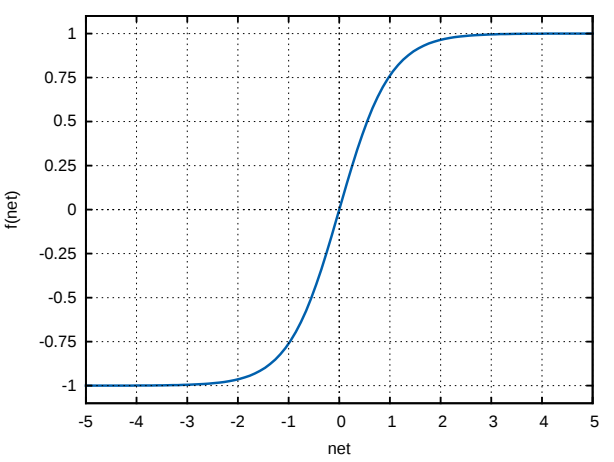
\includegraphics[scale=0.5]{img/tanh-fun.png}
        \caption[Caption for LOF]{Tangens hiperbolni \textit{f(net) = tanh(net)}\footnotemark}
        \label{fig:tanh-fun}
    \end{figure}
    \footnotetext{Preuzeto iz literature \citep{cupicANN}.}
    \item \textbf{Funkcija zglobnica} \engl{ReLU,Rectified Linear Unit} (prikazana na slici \ref{fig:relu-fun}):
    \begin{equation}
        \label{eq:relu}
        relu(net) = max(0, net),
    \end{equation}
    \begin{equation}
        \label{eq:relu-der}
        relu'(net) =
        \begin{cases}
            1, & net > 0\\
            0, & \text{inače}.
        \end{cases}
        .
    \end{equation}
    Iako izgleda kao linearna funkcija, funkcija zglobnica ima svoju derivaciju koja se može koristiti u algoritmu propagacije pogreške unatrag. Računalno je dosta povoljnija od prethodne dvije te je zbog toga danas sve korištenija i to pogotovo tijekom učenja dubokih neuronskih mreža. No, funkcija ima jedan nezgodan problem a to je da "ubija" sve neurone čiji su izlazi jako mali ili negativni te se time učenje u nekim slučajevima izrazito otežava jer gradijent postaje 0. Tom problemu se doskočilo tako da se ipak propuštaju određeni neuroni koji imaju negativne izlaze. Takva funkcija se onda naziva funkcija propusna zglobnica \engl{leaky ReLU} (prikazan na slici \ref{fig:lrelu-fun}) i ima sljedeću definiciju:
    \begin{equation}
        \label{eq:lrelu}
        lrelu(net) = 
        \begin{cases}
            net, & net > 0\\
            \alpha \cdot net, & \text{inače}.
        \end{cases}
        ,
    \end{equation}
    \begin{equation}
        \label{eq:lrelu-der}
        lrelu'(net) =
        \begin{cases}
            1, & net > 0\\
            \alpha, & \text{inače}.
        \end{cases}
        .
    \end{equation}
    $\alpha$ je parametar koji je često jako mali realan broj i u raznim literaturama poprima vrijednosti poput 0.1 i 0.2. Funkcija propusna zglobnica je zgodna, no pokazuje se da ne daje konzistentne rezultate kada mora raditi predikcije negativnih vrijednosti.
    \begin{figure}[H]
        \centering
        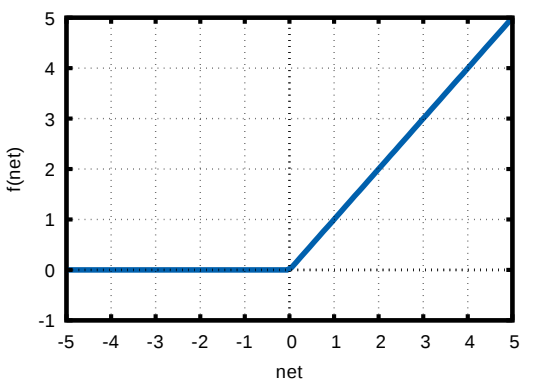
\includegraphics[scale=0.55]{img/relu-fun.png}
        \caption[Caption for LOF]{Funkcija zglobnica \textit{f(net) = relu(net)}\footnotemark}
        \label{fig:relu-fun}
    \end{figure}
    \footnotetext{Preuzeto iz literature \citep{cupicANN}.}
    \begin{figure}[H]
        \centering
        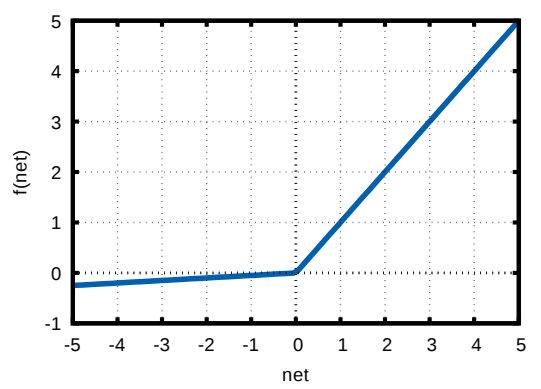
\includegraphics[scale=0.55]{img/lrelu-fun.png}
        \caption[Caption for LOF]{Funkcija propusna zglobnica \textit{f(net) = lrelu(net)}\footnotemark}
        \label{fig:lrelu-fun}
    \end{figure}
    \footnotetext{Preuzeto iz literature \citep{cupicANN}.}
    \item \textbf{Funkcija softmax}: \newline
    Funkcija softmax je funkcija koja ulaze transformira na vrijednost između 0 i 1 baš kao i sigmoidalna funkcija pa je graf praktički identičan te ga nema smisla ponovno prikazivati. No, ideja softmax funkcije je da vrati postotke u kojima se dotični ulazi nalaze i onda suma svih tih postotaka mora biti stopostotna. Koristi se samo kao aktivacijska funkcija izlaznog sloja i vrlo je pogodna kada se radi o problemima višerazredne klasifikacije jer je onda preko postotaka lako za odrediti koji razred se nalazi na izlazu. Definicija funkcije je malo drugačija od ostalih zato što kao ulazni argument prima vektor vrijednosti, a ne samo jednu vrijednost i glasi ovako \citep{softmax}:
    \[
        S(\vec{a}) : \quad
        \begin{bmatrix}
            a\textsubscript{1} \\
            a\textsubscript{2} \\
            \dots \\
            a\textsubscript{N}
        \end{bmatrix}
        \xrightarrow{}
        \begin{bmatrix}
            S\textsubscript{1} \\
            S\textsubscript{2} \\
            \dots \\
            S\textsubscript{N}
        \end{bmatrix} \quad \text{gdje je}
    \]
    \begin{equation}
        \label{eq:soft}
        S\textsubscript{j} = \frac{e^{a\textsubscript{j}}}{\sum\limits_{k=1}^ne^{a\textsubscript{k}}},
    \end{equation}
    \begin{equation}
        \label{eq:soft-der}
        S(\vec{a})' = S(\vec{a}) \cdot (1 - S(\vec{a})).
    \end{equation}
    Vidimo dakle da je i derivacija softmax funkcije gotovo identična derivaciji sigmoidalne, uzevši u obzir da je ulazni argument vektor.
\end{enumerate}

\subsection{Inicijalizacija i normalizacija}
Do sada smo definirali kako za neke ulaze dobiti nekakvu vrstu izlaza koji će biti u rasponu određenom nekom od navedenih aktivacijskih funkcija, no nigdje nismo rekli kakvi ti ulazi trebaju biti. Kojem rasponu brojeva trebaju pripadati? Koje početne vrijednosti trebaju imati težine svih slojeva? Odgovore na ta pitanja ćemo sada pokušati odgovoriti.

\subsubsection{Normalizacija}
Normalizacija \engl{normalization} je postupak kojim se vrijednosti nekih podataka adaptiraju na neki fiksni interval kao npr.\ na interval $(0, 1)$. To je potrebno napraviti prvenstveno jer je tako računalu znatno jednostavnije izvoditi operacije s matricama, a i najčešće na izlazima očekujemo vrijednosti između -1 i 1 pa ako su ulazne vrijednosti puno veće od navedenog, onda mreža vrlo vjerojatno neće dobro naučiti ili će se mučiti da pronađe prave težine. U implementaciji je korišten tip normalizacije u kojoj stvarnu vrijednost ulaza podijelimo maksimalnom mogućom vrijednosti za ulaz. Npr.\ točka koja ima ekranske koordinate x i y će se normalizirati tako da se x koordinata podijeli širinom prozora, dok se y koordinata podijeli visinom prozora.

\subsubsection{Inicijalizacija}
Inicijalizacija \engl{initialization} težina igra još veću ulogu u učenju unaprijedne neuronske mreže od normalizacije ulaza. Zašto nam je uopće potrebna inicijalizacija težina? Pretpostavimo da su sve težine inicijalno postavljene na 0. U tom slučaju će svi neuroni biti simetrični i naučit će iste značajke te zbog toga učenje neće biti moguće. Općenito, bilo kakva inicijalizacija nekom konstantom će rezultirati istim rezultatom. Što će se dogoditi ako težine inicijaliziramo jako velikim, odnosno jako malim brojevima? Ako provedemo takvu inicijalizaciju, dogodit će se problem kojeg nazivamo eksplodirajući, odnosno iščezavajući gradijent. Ako nastupi eksplodirajući gradijent, tada će učenje unaprijedne neuronske mreže drastično divergirati, dok će kod iščezavajućeg gradijenta učenje biti izrazito sporo. Zbog navedenih razloga je vrlo jasno da se težine moraju kvalitetno inicijalizirati. Postoje mnoge metode inicijalizacije, no spomenut ćemo samo onu koja je korištena u implementaciji, a to je Xavier inicijalizacija koja vrijednosti težina generira normalnom razdiobom gdje očekivanje, $\mu$, iznosi 0, a standardna devijacija, $\sigma$, iznosi $\sqrt{\frac{1}{n\textsuperscript{(l-1)}}}$. Nazivnik predstavlja broj neurona u prijašnjem sloju \citep{init}.

\section{Učenje unaprijedne neuronske mreže}
U ovom trenutku trebali bismo biti upoznati s općenitim načinom rada unaprijedne neuronske mreže, a to je aproksimacija, odnosno predikcija nekog izlaza za neki proizvoljan ulaz. Upoznali smo se i s normalizacijom ulaznih podataka, inicijalizacijom težina među neuronima i prikazali smo matematičku interpretaciju svega navedenog. Ostalo nam je još objasniti kako se unaprijedna neuronska mreža uči i to ćemo objasniti u ovom poglavlju.

Unaprijedna neuronska mreža može se učiti na nekoliko načina, a najpoznatiji su učenje algoritmima evolucijskog računanja te učenje algoritmom gradijenti spust i algoritmom propagacije pogreške unatrag. U ovom radu fokus je bio na zadnja dva.

\bigskip

Prije nego što krenemo na algoritam propagacije pogreške unatrag, prisjetimo se kratko koja je temeljna ideja algoritma gradijentni spust.

\subsection{Gradijentni spust}
Gradijentni spust \engl{gradient descent} je algoritam koji se koristi za minimizaciju funkcije pomoću njene derivacije. Pretpostavimo da postoji funkcija $f(x)$ koju želimo minimizirati. Tada ćemo x za koji je funkcija f minimalna tražiti sljedećom formulom:

\begin{equation}
    \label{eq:grad}
    x \leftarrow x - \alpha \cdot{\frac{\partial}{\partial x}}f(x),
\end{equation}

pri čemu je $\alpha$ stopa učenja koja je često mali realan broj. Dan je primjer funkcije s jednom varijablom, no algoritam djeluje i na funkcije s više varijabli. Glavna ideja algoritma je da se po grafu pomičemo u smjeru koji pokazuje na točku gdje će derivacija biti približno jednaka 0, a brzinu kretanja određuje stopa učenja koju smo obradili nešto ranije.

\subsection{Algoritam propagacije pogreške unatrag}
Algoritam propagacije pogreške unatrag \engl{Backpropagation algorithm} je trenutno možda najkorišteniji algoritam učenja unaprijedne neuronske mreže. 1986.\ Rumelhart zajedno s dvojicom prijatelja u svojem radu \textit{Parallel Distributed Processing} po prvi put definira termin \textit{backpropagation} i učenje višeslojnog perceptrona. Oko te godine konektivistički pristup ponovno dobiva zalet i prva zima umjetne inteligencije polako prolazi. U ovom radu nećemo ulaziti previše u detalje izvoda samog algoritma, već ćemo dati općeniti pregled gotovih formula, pseudokod algoritma te neke od inačica. Sve notacije koje smo uveli kod definicije unaprijedne neuronske mreže će vrijediti i ovdje.

Pretpostavimo da imamo skup uzoraka koji se sastoji od \textit{N} različitih uzoraka. Svaki uzorak je predstavljen vektorom ulaza i vektorom očekivanih izlaza i označimo ga kao $(x\textsubscript{s,1}, x\textsubscript{s,2},\dots, x\textsubscript{s,n}) \xrightarrow{} (d\textsubscript{s,1}, d\textsubscript{s,2},\dots, d\textsubscript{s,m})$, gdje su ulazi označeni slovom \textbf{x}, a željeni izlazi slovom \textbf{d}. Indeks \textit{s} predstavlja \textit{s}-ti uzorak, a \textit{n} i \textit{m} broj neurona na ulazu, odnosno na izlazu neuronske mreže.\footnote{Pogledaj sliku \ref{fig:ann}.} Također, pretpostavimo da je mreža sastavljena od \textit{L} slojeva gdje je \textit{L}-ti sloj izlazni sloj. Da bi mreža mogla učiti, moramo definirati određenu funkciju kazne pomoću koje će mreža dobiti povratnu informaciju o tome koliko dobro ili loše uči te na temelju te pogreške korigirati iznose težina. Funkcija kazne za jedan uzorak definirana je na sljedeći način:

\begin{equation}
    \label{eq:sample-err}
    E(s) = \frac{1}{2}\sum\limits_{i=1}^m(d\textsubscript{s,i} - y\textsubscript{s,i}\textsuperscript{(L)})^2.
\end{equation}

S obzirom na to da želimo učiti nad cijelim skupom uzoraka, onda je potrebno definirati funkciju kazne nad cijelim skupom uzoraka:

\begin{equation}
    \label{eq:err}
    E = \frac{1}{N}\sum\limits_{s=1}^NE(s) = \frac{1}{2N}\sum\limits_{s=1}^N\sum\limits_{i=1}^m(d\textsubscript{s,i} - y\textsubscript{s,i}\textsuperscript{(L)})^2.
\end{equation}

Ako se prisjetite formule za izračun izlaza neurona pomoću net vrijednosti i aktivacijske funkcije, onda vrlo lako možemo zaključiti da funkcija kazne ovisi o težinama jer svaki izlaz ovisi o težinama i ulazima prijašnjeg sloja, a svaki ulaz je zapravo izlaz prijašnjeg sloja pa onda i on posljedično ovisi o težinama i tako sve do prvog skrivenog sloja:

\[
    \vec{y}\textsuperscript{ (L)} = g(\textbf{W\textsuperscript{(L--1)}} \cdot{\vec{y}\textsuperscript{ (L--1)}} + \vec{b}\textsuperscript{ (L--1)}),
\]
\[
    \vec{y}\textsuperscript{ (L--1)} = g(\textbf{W\textsuperscript{(L--2)}} \cdot{\vec{y}\textsuperscript{ (L--2)}} + \vec{b}\textsuperscript{ (L--2)}),
\]
\[
    \dots
\]
\[
    \vec{y}\textsuperscript{ (2)} = g(\textbf{W\textsuperscript{(1)}} \cdot{\vec{y}\textsuperscript{ (1)}} + \vec{b}\textsuperscript{ (1)}).
\]

Sada kada to znamo, onda je potrebno minimizirati funkciju, tj.\ algoritmom gradijentni spust pronaći one težine za koje je funkcija kazne minimalna:

\begin{equation}
    \label{eq:weight-grad}
    w\textsubscript{jk}\textsuperscript{(l)} \leftarrow  w\textsubscript{jk}\textsuperscript{(l)} - \alpha \cdot{\frac{\partial E}{\partial w\textsubscript{jk}\textsuperscript{(l)}}}.
\end{equation}

Možda se sada pitate zašto nam je potreban backpropagation algoritam kada očigledno gradijenti spusta možemo direktno primijeniti. Ta pretpostavka je u redu u slučaju kada nemamo mnoštvo uzoraka za učenje i kada arhitektura mreže nije kompleksna, no što ako imamo desetke tisuća uzoraka s nekoliko skrivenih slojeva gdje svaki ima minimalno deset neurona? Tada bi računanje jedne po jedne težine bilo izrazito računalno zahtjevno i sporo, a to želimo izbjeći. Upravo zbog navedenog koristimo backpropagation algoritam jer njime uvelike olakšavamo izračun parcijalnih derivacija za sve težine, a time i samo učenje mreže.

Kada smo govorili o ADALINE neuronu, spomenuli smo da se on, kao i MCP neuron, uče delta pravilom. Delta pravilom je moguće učiti samo jednoslojne perceptrone, stoga se ono moralo malo nadograditi tako da se može koristiti za učenje višeslojnog perceptrona.

% \begin{description}
%     \item[$\delta$\textsubscript{j}\textsuperscript{(l)} :] pogreška između očekivanog i stvarnog izlaza j-tog neurona l-tog sloja,
%     \item[$\vec{\delta}$\textsuperscript{ (l)} :] vektora pogrešaka l-tog sloja,
% \end{description}

Pokažimo kako bi izgledala parcijalna derivacija funkcije kazne u zadnjem sloju prije izlaznog:

\begin{align}
    \label{eq:4-26}
    \frac{\partial E}{\partial w\textsubscript{jk}\textsuperscript{(L--1)}} &= \frac{\partial}{\partial w\textsubscript{jk}\textsuperscript{(L--1)}}\left[\frac{1}{2N}\sum\limits_{s=1}^N\sum\limits_{i=1}^m(d\textsubscript{s,i} - y\textsubscript{s,i}\textsuperscript{(L)})^2\right] \\
    &= \frac{1}{2N}\sum\limits_{s=1}^N\sum\limits_{i=1}^m2\cdot{(d\textsubscript{s,i} - y\textsubscript{s,i}\textsuperscript{(L)}}) \cdot{(-1)} \cdot{\frac{\partial y\textsubscript{s,i}\textsuperscript{(L)}}{\partial w\textsubscript{jk}\textsuperscript{(L--1)}}} \\
    &= -\frac{1}{N}\sum\limits_{s=1}^N\sum\limits_{i=1}^m(d\textsubscript{s,i} - y\textsubscript{s,i}\textsuperscript{(L)})\cdot{\frac{\partial y\textsubscript{s,i}\textsuperscript{(L)}}{\partial w\textsubscript{jk}\textsuperscript{(L--1)}}}
\end{align}

S obzirom na to da težina w\textsubscript{jk}\textsuperscript{(L--1)} utječe samo na y\textsubscript{s,j}\textsuperscript{(L)}, onda svaka parcijalna derivacija $\frac{\partial y\textsubscript{s,i}\textsuperscript{(L)}}{\partial w\textsubscript{jk}\textsuperscript{(L--1)}}$ za slučaj da je $i\neq{j}$ iščezava te vrijedi:
\[
    \sum\limits_{i=1}^m\frac{\partial y\textsubscript{s,i}\textsuperscript{(L)}}{\partial w\textsubscript{jk}\textsuperscript{(L--1)}} = \frac{\partial y\textsubscript{s,j}\textsuperscript{(L)}}{\partial w\textsubscript{jk}\textsuperscript{(L--1)}}.
\]
Dakle, sada možemo pisati:
\begin{equation}
    \label{eq:4-27}
    \frac{\partial E}{\partial w\textsubscript{jk}\textsuperscript{(L--1)}} = -\frac{1}{N}\sum\limits_{s=1}^N(d\textsubscript{s,j} - y\textsubscript{s,j}\textsuperscript{(L)})\cdot{\frac{\partial y\textsubscript{s,j}\textsuperscript{(L)}}{\partial w\textsubscript{jk}\textsuperscript{(L--1)}}}
\end{equation}

Preostalu parcijalnu derivaciju možemo riješiti pomoću pravila ulančavanja:
\begin{equation}
    \frac{\partial y\textsubscript{s,j}\textsuperscript{(L)}}{\partial w\textsubscript{jk}\textsuperscript{(L--1)}} = \frac{\partial y\textsubscript{s,j}\textsuperscript{(L)}}{\partial net\textsubscript{s,j}\textsuperscript{(L)}} \cdot \frac{\partial net\textsubscript{s,j}\textsuperscript{(L)}}{\partial w\textsubscript{jk}\textsuperscript{(L--1)}},
\end{equation}

gdje vrijedi sljedeće:
\begin{equation}
    \frac{\partial y\textsubscript{s,j}\textsuperscript{(L)}}{\partial net\textsubscript{s,j}\textsuperscript{(L)}} = \frac{\partial g(net\textsubscript{s,j}\textsuperscript{(L)})}{\partial net\textsubscript{s,j}\textsuperscript{(L)}} = g'(net\textsubscript{s,j}\textsuperscript{(L)}),
\end{equation}
\begin{equation}
    \frac{\partial net\textsubscript{s,j}\textsuperscript{(L)}}{\partial w\textsubscript{jk}\textsuperscript{(L--1)}} = \frac{\partial}{\partial w\textsubscript{jk}\textsuperscript{(L--1)}}(w\textsubscript{j1}\textsuperscript{(L--1)}\cdot y\textsubscript{s,1}\textsuperscript{(L--1)} + \dots + w\textsubscript{jk}\textsuperscript{(L--1)}\cdot y\textsubscript{s,k}\textsuperscript{(L--1)} + \dots) = y\textsubscript{s,k}\textsuperscript{(L--1)}.
\end{equation}

Nakon uvrštavanja u izraz \eqref{eq:4-27} dobivamo:
\begin{align}
    \frac{\partial E}{\partial w\textsubscript{jk}\textsuperscript{(L--1)}} &= -\frac{1}{N}\sum\limits_{s=1}^N g'(net\textsubscript{s,j}\textsuperscript{(L)})\cdot(d\textsubscript{s,j} - y\textsubscript{s,j}\textsuperscript{(L)})\cdot y\textsubscript{s,k}\textsuperscript{(L--1)} \\
    &= -\frac{1}{N}\sum\limits_{s=1}^N \delta\textsubscript{s,j}\textsuperscript{(L)} \cdot y\textsubscript{s,k}\textsuperscript{(L--1)},
\end{align}

gdje je $\delta\textsubscript{s,j}\textsuperscript{(L)}$ pogreška j-tog neurona s-tog uzorka na izlaznom sloju i definira se kao:
\begin{equation}
    \label{eq:delta-izlaz}
    \delta\textsubscript{s,j}\textsuperscript{(L)} = g'(net\textsubscript{s,j}\textsuperscript{(L)})\cdot(d\textsubscript{s,j} - y\textsubscript{s,j}\textsuperscript{(L)}).
\end{equation}
Sada kada smo definirali parcijalnu derivaciju za proizvoljnu težinu zadnjeg skrivenog sloja, ažuriranje težina na temelju \eqref{eq:weight-grad} glasi:
\begin{align}
    w\textsubscript{jk}\textsuperscript{(L--1)} &\leftarrow w\textsubscript{jk}\textsuperscript{(L--1)} - \alpha\cdot \left(-\frac{1}{N}\sum\limits_{s=1}^N \delta\textsubscript{s,j}\textsuperscript{(L)} \cdot y\textsubscript{s,k}\textsuperscript{(L-1)}\right) \\
    &\leftarrow w\textsubscript{jk}\textsuperscript{(L--1)} + \eta\cdot\sum\limits_{s=1}^N \delta\textsubscript{s,j}\textsuperscript{(L)} \cdot y\textsubscript{s,k}\textsuperscript{(L--1)}
\end{align}
gdje smo umjesto $\alpha \cdot \frac{1}{N}$ uveli konstantu $\eta$ za koju i dalje vrijede svojstva koje smo naveli za stopu učenja.

\bigskip

Postupak koji smo proveli vrijedi kada tražimo parcijalne derivacije za težine predzadnjeg sloja, no procedura za ostale slojeve je gotovo pa identična. Postupak se počinje mijenjati u formuli \eqref{eq:4-26}:
\begin{equation}
    \frac{\partial E}{\partial w\textsubscript{jk}\textsuperscript{(L--2)}} =
    -\frac{1}{N}\sum\limits_{s=1}^N\sum\limits_{i=1}^m(d\textsubscript{s,i} - y\textsubscript{s,i}\textsuperscript{(L)})\cdot{\frac{\partial y\textsubscript{s,i}\textsuperscript{(L)}}{\partial w\textsubscript{jk}\textsuperscript{(L--2)}}},
\end{equation}
gdje navedenu parcijalnu derivaciju opet rješavamo pravilom ulančavanja. Ako detaljnije raspišemo, onda ćemo vidjeti da će biti potrebno "spustiti" se do (L--2)-vog sloja. Konačna formula za pogrešku j-tog neurona (L--1)-vog sloja i ažuriranje težina će onda glasiti: 
\begin{equation}
    \label{eq:delta-ostali}
    \delta\textsubscript{s,j}\textsuperscript{(L--1)} = g'(net\textsubscript{s,j}\textsuperscript{(L--1)})\cdot\sum\limits_{i=1}^m\delta\textsubscript{s,i}\textsuperscript{(L)}\cdot w\textsubscript{i,j}\textsuperscript{(L--1)},
\end{equation}
\begin{equation}
    w\textsubscript{jk}\textsuperscript{(L--2)} \leftarrow w\textsubscript{jk}\textsuperscript{(L--2)} + \eta\cdot\sum\limits_{s=1}^N \delta\textsubscript{s,j}\textsuperscript{(L--1)} \cdot y\textsubscript{s,k}\textsuperscript{(L--2)}.
\end{equation}

\begin{algorithm}
\caption{Backpropagation algoritam\footnotemark}
\label{algo:alg-backprop}
    \begin{enumerate}
        \item[\textbf{1.}] Ciklički prolazi kroz svih \textit{N} uzoraka za učenje, jedan po jedan.
        \item[\textbf{2.}] Ponavljaj dok nije zadovoljen uvjet zaustavljanja.
        \item[\textbf{3.}] Za svaki uzorak iz skupa uzoraka za učenje čini:
        \begin{enumerate}
            \item[\textbf{1.}] Postavi uzorak na ulaz unaprijedne neuronske mreže i izračunaj izlaze za sve neurone primjenom formule \eqref{eq:izlaz-matrice}.
            \item[\textbf{2.}] Izračunaj pogrešku svakog od neurona izlaznog sloja po formuli \eqref{eq:delta-izlaz}.
            \item[\textbf{3.}] Vraćaj se sloj po sloj i izračunaj pogreške svakog neurona po formuli \eqref{eq:delta-ostali}.
            \item[\textbf{4.}] Ažuriraj težine po formuli:
                \begin{equation}
                    \label{eq:azuriranje}
                    w\textsubscript{jk}\textsuperscript{(l)} \leftarrow w\textsubscript{jk}\textsuperscript{(l)} + \eta\cdot\sum\limits_{s=1}^N \delta\textsubscript{s,j}\textsuperscript{(l+1)} \cdot y\textsubscript{s,k}\textsuperscript{(l)}.
                \end{equation}
            \item[\textbf{5.}] Ažuriraj biase po formuli (prisjetite se da su ulazi konstantni):
                \begin{equation}
                    \label{eq:azuriranje-bias}
                    b\textsubscript{j}\textsuperscript{(l)} \leftarrow b\textsubscript{j}\textsuperscript{(l)} + \eta\cdot\sum\limits_{s=1}^N \delta\textsubscript{s,j}\textsuperscript{(l+1)}.
                \end{equation}
        \end{enumerate}
    \end{enumerate}
\end{algorithm}
\footnotetext{Iz literature \citep{cupicANN}.}

\newpage
Dakle, uvjerili smo se da će izračuni parcijalnih derivaciju uz pomoć backpropagation algoritma biti znatno brži, nego da smo ih pojedinačno računali. Za jednu epohu učenja kroz mrežu je potrebno proći svega dva puta: algoritmom unaprijedne neuronske mreže te backpropagation algoritmom, što je vrlo efikasno. Također, uvjet zaustavljanja učenja može biti da funkcija kazne poprimi određeni error kojeg korisnik izvana zada ili jednostavno da se učenje završi nakon određenog broja epoha.

\bigskip

Spomenimo još tri glavna tipa učenja backpropagation algoritmom, a to su:
\begin{enumerate}
    \item Skupno učenje \engl{batch learning} - težine se ažuriraju tek kada kroz mrežu prođu svi uzorci, vremenski je dosta zahtjevan, ali je jako precizan.
    \item Učenje po manjim grupama \engl{mini-batches learning} - težine se ažuriraju nakon što kroz mrežu prođe određen broj uzoraka, vremenski je manje zahtjevan od skupnog, ali je manje precizan.
    \item Stohastičko učenje \engl{stochastic learning} - težine se ažuriraju nakon svakog uzorka, vremenski je najpovoljnije, ali je nešto neprecizniji od mini-batchesa. Često se naziva i \textit{online} učenje zbog ažuriranja nakon svakog uzorka.
\end{enumerate}

\bigskip
\bigskip

U sljedećem poglavlju ćemo pokazati rezultate programske implementacije.

\chapter{Rezultati}
Programska implementacija ovog rada pisana je programskim jezikom \textit{Java} verzije \textit{13} i pomoćnog alata \textit{Maven} verzije \textit{3.6.3}. Korištena je samo jedna eksterna biblioteka za rad s matricama\footnote{\textit{Apache Commons Math} 3.6.1 \url{http://commons.apache.org/proper/commons-math/}.}, dok je sve ostalo pisano standardnim Javinim bibliotekama kao npr.\ \textit{Swing}.

U sklopu implementacije implementirana je unaprijedna neuronska mreža razredom \textit{NeuralNetwork} koji posjeduje metodu \textit{feedForward} zaslužnu za dobivanje izlaza za neki ulaz te metodu \textit{train} koja trenira istu backpropagation algoritmom. U nastavku su prikazane signature metoda.
\begin{lstlisting}
public class NeuralNetwork {
    ...
    public double[] feedForward(double[] inputs) {...}
    public void train(
        int epochs, double maxError, double eta) {...}
    ...
}
\end{lstlisting}
Također, implementirano je i jedno grafičko korisničko sučelje (\textit{GUI}) koje je prikazano na slici \ref{fig:gui}. GUI je dosta samodokumentirajući, ali spomenimo par sitnica. Mreži se za učenje predaju uzorci iz 2D koordinatnog sustava koji se unose klikom lijevog miša, dok se klikom desnog miša mijenja tip razreda kao što je navedeno pod \textbf{Class type}. Mogu se izabrati tri tipa backpropagation algoritma koje smo spomenuli ranije. S obzirom na to da mreža ima fiksne ulaze (2 ulaza: x i y koordinata točke) i fiksne izlaze (3 izlaza jer su omogućene tri vrste razreda), omogućeno je postavljanje samo skrivenih slojeva. Ostale karakteristike sučelja bi trebale biti jasne. Potvrdimo teoriju ovog rada na temelju sljedećih nekoliko primjera.

\begin{figure}[H]
    \centering
    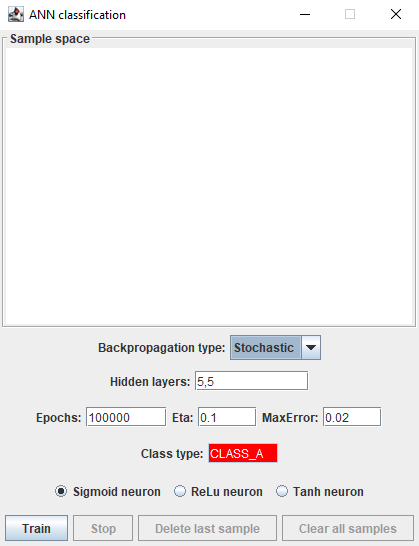
\includegraphics[scale=0.6]{img/gui.png}
    \caption[Caption for LOF]{Grafičko korisničko sučelje}
    \label{fig:gui}
\end{figure}

Krenimo s jednoslojnim perceptronom i linearnom klasifikacijom prikazanom na slici \ref{fig:single-layer-class}. Korištena aktivacijska funkcija u ovom slučaju je ReLU, no sve tri navedene daju donekle sličan rezultat što se tiče oblika decizijske granice jer se radi o linearnoj klasifikacija gdje nema previše mudrovanja.

\begin{figure}[H]
    \centering
    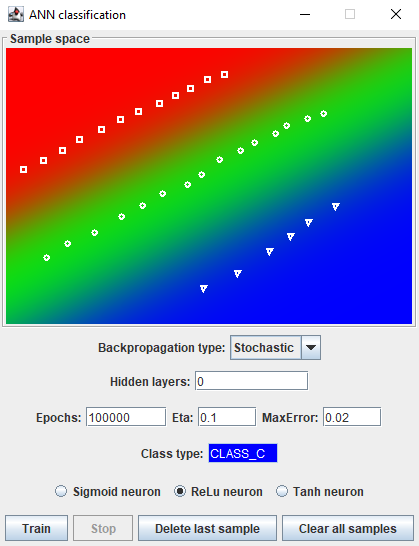
\includegraphics[scale=0.6]{img/single-layer.png}
    \caption[Caption for LOF]{Linearna klasifikacija - jednoslojni perceptron}
    \label{fig:single-layer-class}
\end{figure}

Pogledajmo što će se dogoditi ako problem nije linearno interpretabilan i ako koristimo jednoslojni perceptron. Rezultat je prikazan na slici \ref{fig:single-layer-fail}. Vidimo da je klasifikator neke točke dobro klasificirao, a neke nije te smo time upravo dokazali da jednoslojni perceptron nije u stanju kvalitetno riješiti probleme koji nisu linearno interpretabilni.

\begin{figure}[H]
    \centering
    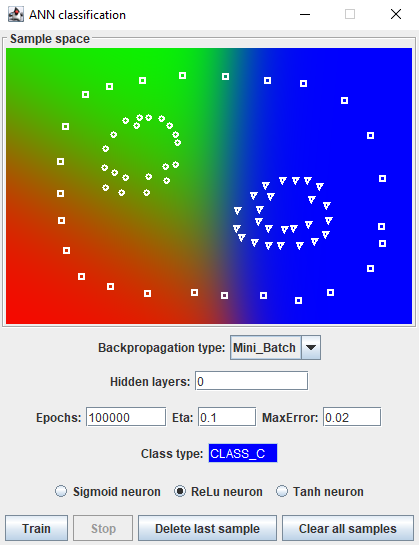
\includegraphics[scale=0.6]{img/single-layer-fail.png}
    \caption[Caption for LOF]{Nelinearna klasifikacija - jednoslojni perceptron}
    \label{fig:single-layer-fail}
\end{figure}

Pogledajmo sada kako bi višeslojni perceptron riješio isti problem. Rezultat je prikazan na slici \ref{fig:tanh-multilayer}. Korišten je tangens hiperbolni kao aktivacijska funkcija jer je davala najbolje rezultate za trenutni problem i korišten je tip učenja u grupama (\textit{mini-batches}) gdje se svaka grupa sastoji od maksimalno 30 uzoraka. Arhitektura mreže sada glasi 2x5x3, što znači da smo dodali jedan skriveni sloj od 5 neurona. No, i dalje nismo zadovoljni kako klasifikator radi pa probajmo mrežu učiniti još ekspresivnijom dodavši joj još slojeva i neurona.

Na slici \ref{fig:relu-multilayer} prikazani su nešto bolji rezultati nego ranije jer smo mrežu učinili nešto ekspresivnijom dodavši joj još jedan skriveni sloj od 5 neurona i promijenivši tip backpropagation algoritma u stochastic kao i aktivacijsku funkciju u ReLU. Također, možemo vidjeti kako ReLU funkcija utječe na izgled decizijskih granica čineći grupirane razrede kao pravokutne likove. Pogledajmo možemo li klasifikator još bolje naučiti. Ispostavlja se da možemo, no što je mreža ekspresivnija time će se klasifikator pretrenirati samo nad uzorcima za učenje te time neće razviti svojstvo generalizacije i neće biti primjenjiv izvan predstavljenog problema, a to je jako loša praksa. Rezultati su prikazani na slikama \ref{fig:sigmoid-almost-best} i \ref{fig:overfitting}. Uočite arhitekture neuronske mreže kao i maksimalan error za koji se prekida učenje.

\begin{figure}[H]
    \centering
    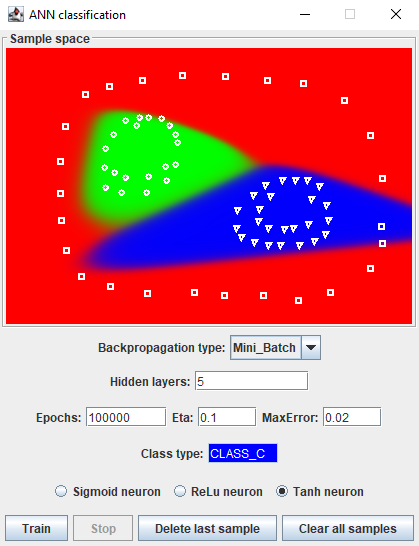
\includegraphics[scale=0.6]{img/tanh-better.png}
    \caption[Caption for LOF]{Nelinearna klasifikacija - višeslojni perceptron}
    \label{fig:tanh-multilayer}
\end{figure}

\begin{figure}[H]
    \centering
    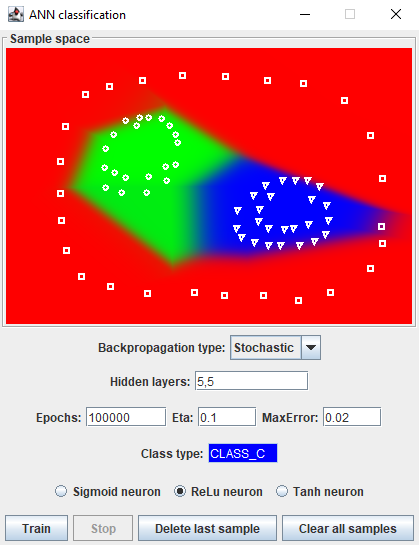
\includegraphics[scale=0.6]{img/relu-better-better.png}
    \caption[Caption for LOF]{Nelinearna klasifikacija - bolje}
    \label{fig:relu-multilayer}
\end{figure}

\begin{figure}[H]
    \centering
    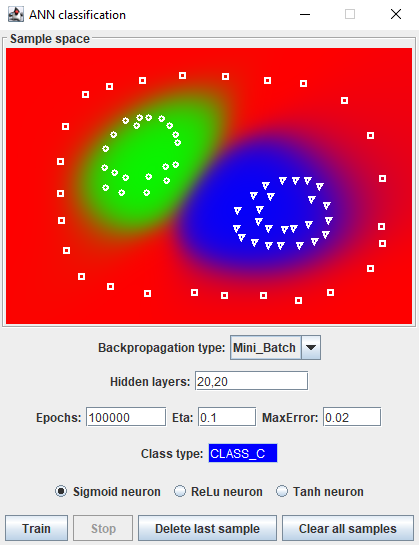
\includegraphics[scale=0.6]{img/sigmoid-almost-best.png}
    \caption[Caption for LOF]{Nelinearna klasifikacija - još bolje}
    \label{fig:sigmoid-almost-best}
\end{figure}

\begin{figure}[H]
    \centering
    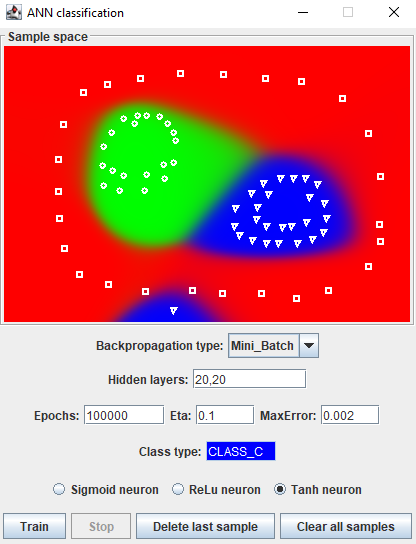
\includegraphics[scale=0.6]{img/overfitting.png}
    \caption[Caption for LOF]{Pretreniranost}
    \label{fig:overfitting}
\end{figure}

\chapter{Zaključak}
Kroz ovaj rad obrađen je algoritam unaprijedne umjetne neuronske mreže i učenje iste algoritmom propagacije pogreške unatrag.

Najveći problem u realizaciji jednog takvog algoritma predstavlja upravo pametna inicijalizacija težina među neuronima, izbor aktivacijskih funkcija i arhitektura same mreže. Često moramo jako dobro poznavati teoriju koja se krije iza kulisa da bi se mogli suočiti s mnoštvom različitih problema na prihvatljiv način, inače možemo unedogled vrtjeti algoritam bez kvalitetnih rezultata.

Unatoč svemu, implementacija ovog rada je dosta uspješno realizirana i model klasifikatora za različite aktivacijske funkcije daje dosta dobre rezultate.

\bigskip
Za daljnji nastavak ovog rada bi se moglo proučiti mnoštvo različitih inačica backpropagation algoritma u svrhu postizanja boljih rezultata i upoznati se s dubokim neuronskim mrežama i algoritmima dubokog učenja.

\bibliography{literatura}
\bibliographystyle{fer}

\begin{sazetak}
Raspoznavanje uzoraka te klasifikacija istih je jedan od bitnijih problema računarske znanosti. Najveći izazov je konstruirati kvalitetan klasifikator koji je sposoban generalizirati. U ovom radu prikazan je teorijski pogled na algoritam umjetne neuronske mreže kroz povijest pa do danas i njegovo učenje backpropagation algoritmom. Također, uz rad je i implementirano jedno takvo učenje kroz grafičko korisničko sučelje kroz koje korisnik interaktivno unosi točke iz 2D koordinatnog sustava labelirane različitim razredima i prati koliko kvalitetno klasifikator uči. Reprezentativni rezultati prikazani su i dokumentirani u radu.

\kljucnerijeci{Nadzirano učenje, klasifikacija, unaprijedna neuronska mreža, algoritam propagacije pogreške unatrag, aktivacijska funkcija, umjetni neuron.}
\end{sazetak}

\engtitle{Classification Based on Artificial Neural Networks}
\begin{abstract}
Pattern recognition and classification is one of the most important problem in computer science. The biggest challenge is to construct a good classifier that is capable of generalizing. This paper presents a theoretical view of the artificial neural network algorithm through history to the present day and its learning by the backpropagation algorithm. Also, in addition to the work, one such learning was implemented through a graphical user interface through which the user interactively enters points from the 2D coordinate system labeled with different classes and monitors how well the classifier learns. Representative results are presented and documented in the paper.

\keywords{Supervised learning, classification, feedforward neural network, backpropagation, activation function, artificial neuron.}
\end{abstract}

\end{document}
